% Možné jazyky práce: czech, english
% Možné typy práce: BP (bakalářská), DP (diplomová)
\documentclass[czech,DP]{thesiskiv}

\author{Bc. David Pivovar}
\declarationmale

% Název práce
\title{Detekce vybraných aktivit diabetického pacienta 1.~typu}

% 
% Texty abstraktů (anglicky, česky)
%
\abstracttexten{
This thesis deals with carbohydrate and physical activity detection of a type 1 diabetic patient. The aim of the thesis was to evaluate existing detection methods and implement detection as filters in the SmartCGMS application. Two methods were proposed and implemented for carbohydrate detection. The first method uses recurrent neural networks, while the second detects the edges of the interstitial glucose waveform measured by a continuous glucose monitoring sensor. Physical activity detection is based on heart rate and motion data.
}

\abstracttextcz{
Tato diplomová práce se zabývá detekcí karbohydrátů a fyzické aktivity diabetického pacienta 1. typu. Cílem práce bylo zhodnotit existující metody detekce a implementovat vlastní řešení jako filtry do aplikace SmartCGMS. Pro detekci karbohydrátů byly navrženy a implementovány dvě metody. První využívá rekurentní neuronové sítě, druhá detekuje hrany průběhu intersticiální glukózy měřené senzorem kontinuální monitorace glukózy. Detekce fyzické aktivity je na základě hodnot srdečního tepu a pohybových dat.
}

% Na titulní stranu a do textu prohlášení se automaticky vkládá 
% aktuální rok, resp. datum. Můžete je změnit:
%\titlepageyear{2016}
%\declarationdate{1. března 2016}

% Ve zvláštních případech je možné ovlivnit i ostatní texty:
%
%\university{Západočeská univerzita v Plzni}
%\faculty{Fakulta aplikovaných věd}
%\department{Katedra informatiky a výpočetní techniky}
%\subject{Bakalářská práce}
%\titlepagetown{Plzeň}
%\declarationtown{Plzni}

%%%%%%%%%%%%%%%%%%%%%%%%%%%%%%%%%%%%%%%%%%%%%%%%%%%%%%%%%%
%
% DODATEČNÉ BALÍČKY PRO SAZBU
% Jejich užívání či neužívání záleží na libovůli autora 
% práce
%
%%%%%%%%%%%%%%%%%%%%%%%%%%%%%%%%%%%%%%%%%%%%%%%%%%%%%%%%%%

% Zařadit literaturu do obsahu
\usepackage[nottoc,notlot,notlof]{tocbibind}

% Umožňuje vkládání obrázků
\usepackage[pdftex]{graphicx}
\usepackage{float}
\usepackage{rotating}

% Odkazy v PDF jsou aktivní; navíc se automaticky vkládá
% balíček 'url', který umožňuje např. dělení slov
% uvnitř URL
\usepackage[pdftex,]{hyperref}
\hypersetup{colorlinks=true,
  unicode=true,
  linkcolor=black,
  citecolor=black,
  urlcolor=black,
  bookmarksopen=true}
  
\usepackage{pdfpages}

% Při používání citačního stylu csplainnatkiv
% (odvozen z csplainnat, http://repo.or.cz/w/csplainnat.git)
% lze snadno modifikovat vzhled citací v textu
\usepackage[numbers,sort&compress]{natbib}
\usepackage{amsmath}

\usepackage{adjustbox}

%%%%%%%%%%%%%%%%%%%%%%%%%%%%%%%%%%%%%%%%%%%%%%%%%%%%%%%%%%
%
% VLASTNÍ TEXT PRÁCE
%
%%%%%%%%%%%%%%%%%%%%%%%%%%%%%%%%%%%%%%%%%%%%%%%%%%%%%%%%%%
\begin{document}
%
\maketitle
\tableofcontents
\parskip=6pt

\chapter{Úvod}

Diabetes mellitus je rozšířené chronické metabolické onemocnění. Vyznačuje se zvýšenou koncentrací cukru v krvi (glykémie), která vniká z nedostatku inzulinu nebo rezistencí vůči jeho působení. Hlavní součástí léčby je monitorace koncentrace glukózy a podávání inzulinu. V dnešní době je možné sledovat vývoj glykémie díky sytémům kontinuální monitorace glukózy (CGMS) a kontinuálnímu dávkování inzulinu díky inzulinovým pumpám. Integrace těchto dvou systémů umožňuje autonomní řízení dávkování inzulinu v závislosti na aktuální koncentraci glukózy.

Koncentraci glukózy v krvi ovlivňuje mnoho faktorů. Dva nejvýznamnější faktory jsou příjem karbohydrátů a fyzická aktivita. Tyto aktivity je třeba kompenzovat zvýšením či snížením množství podávaného inzulinu. Aktuálně je do CGMS zadává pacient a dávku inzulinu upravuje také on. Monitorace těchto aktivit slouží pro správné nastavení léčby diabetologem. Jejich včasná detekce by umožnila přesnější monitoraci vývoje glykémie a lepší řízení autonomních systémů s minimálním zásahem pacienta.

V mé práci se budu zabývat možnostmi detekce příjmu kabohydrátů a fyzické aktivity z dat senzoru CGMS. Následně tyto metody implementuji do aplikace SmartCGMS vyvíjené na katedře informatiky a výpočetní techniky na ZČU.
\chapter{Diabetes mellitus}

Diabetes mellitus je chronické metabolické onemocnění. Vyznačuje se zvýšenou hladinou cukru v krvi, která se nazývá hyperglykémie. V normálu je hladina glykémie (koncentrace glukózy v krvi) mezi 3,8 a 5,6 mmol/l. Po jídle může glykémie stoupnout, neměla by však přesáhnout 7,8 mmol/l. O diabetes se jedná pokud jsou hodnoty vyšší než 11,1 mmol/l.

Hyperglykémie vzniká z nedostatku inzulinu nebo rezistencí buněk vůči jeho působení. Inzulin je hormon, který se tvoří v beta buňkách Langerhansových ostrůvků ve tkáni slinivky břišní. Tento hormon slouží k transportu glukózy z krve do tkáně, kde je využita k tvorbě energie nebo se zde ukládá ve formě glykogenu (v játrech) a tuků. Snižuje tak hladinu cukru v krevním řečišti. Pokud je hladina cukru nízká, produkce inzulinu se okamžitě zastaví  a hormony glukagon a adrenalin uvolní glukózu ze zásobních zdrojů pro zajištění fungování důležitých orgánů, především mozku, nervů a svalů.

Nedostatek inzulinu vede k nedostatečné utilizaci glukózy, která se hromadí v krvi. Dochází k poruše tvorby bílkovin, zvýšené tvorbě ketolátek, které se hromadí a způsobují překyselení organismu, a celkovému metabolickému rozvratu. Při hladině glykémie vyšší než 10-12 mmol/l začnou ledviny uvolňovat glukózu do moči spolu s dalšími látkami a vodou. To vše vyvolává dehydrataci, nevolnost, pokles krevního tlaku, poruchy vědomí.

Dlouhodobě přetrvávající hyperglykémie vede k poškození orgánů, především cév, nervového systému, ledvin a očí. Poškozením velkých cév může dojít k srdečnímu infarktu, mozkové příhodě nebo uzavření tepen v oblasti dolních končetin (ischemická choroba dolních končetin). U diabetických pacientů mají tato onemocnění komplikovanější průběh a vyšší úmrtnost. Nervové poškození je označováno jako diabetická neuropatie. Nejčastěji se objevuje v oblasti dolních končetin. končetina ztrácí citlivost, kůže vysychá a tvoří se defekt do kterého se snadno dostane infekce. Pokud není včas léčen, rozvíjí se syndrom diabetické nohy, který může vést k amputaci končetiny. poškození ledvin může vést k dialýze až k transplantaci ledvin. Poškození očí je příčinou vzniku šedého zákalu.

Bez léčby inzulinem může toto onemocnění vést k smrti. \cite{Diabetes.Psottova,Wikiskripta,cukrovka.cz,Diabetes.TaiN}


\section{Dělení diabetu}

Diabetes se dělí do čtyř základních skupin: diabetes 1. typu, diabetes 2. typu, gestační (těhotenský) diabetes, jiné specifické typy diabetu.

Diabetes mellitus 1. typu je autoimunitní onemocnění kdy vlastní imunitní systém zničí beta buňky Langerhansových ostrůvků produkující inzulin. Při zničení 75-85\% je absolutní nedostatek inzulinu a objevují se zvýšené hodnoty glykémie. Diabetes 1. typu se nejčastěji projeví již v dětském věku, ale může dlouho probíhat v latentní formě a projevit se až v pozdějším věku (LADA - latentní autoimunitní diabetes u dospělých). Že se jedná o LADA a ne diabetes 2. typu se určí detekcí autoprotilátek, které vznikají při poškozování beta buněk. Nemoc se projevuje častým močením, hubnutím a celkovou slabostí. Příčina vzniku diabetu 1. typu není známá a vlohy jsou často dědičné. Protože příčina vzniku není známa, není žádná účinná prevence.

Diabetes mellitus 2. typu je metabolickou poruchou kdy jsou buňky rezistentní vůči vlastnímu inzulinu, tj. buňky nejsou schopny vychytat inzulin v krevním oběhu, který by použili ke zpracování glukózy a úpravě hladiny glykémie. V počátcích beta buňky slinivky břišní reagují zvýšenou produkcí inzulinu (bezpříznaková inzulinová rezistence). Postupem času ale nejsou schopny dodávat potřebné množství inzulinu, nastává relativní nedostatek inzulinu a vzniká prediabetes a diabetes 2. typu. Příznaky jsou únava, žízeň, časté močení, pocit hladovění, hubnutí, infekce, špatné hojení a zhoršení zraku. Diabetes mellitus 2. typu vzniká v dospělosti na základě genetických předpokladů (inzulinová rezistence, nízká produkce inzulinu), rizikových faktorů a špatného životního stylu. Mezi ty patří nedostatek pohybu, nezdravá strava, nadváha a obezita (90\% diabetiků 2. typu trpí nadváhou nebo je obézních), kouření, vysoká hladina cholesterolu a vysoký krevní tlak (hypertenze).

Gestační diabetes se objevuje v druhé polovině těhotenství a končí po porodu. Postihuje 17\% těhotných žen, které k ní mají vrozenou dispozici. Neléčený diabetes má negativní dopad na vývoj plodu, který se musí vyrovnat se zvýšeným přísunem glukózy. Plod, který má produkci inzulinu v pořádku, pak výrazně rychleji roste. To může vést k předčasnému porodu, vrozeným vývojovým vadám, dechovým obtížím, poruchám srdečního rytmu, poruchám vývoje mozku, sklon k obezitě a rozvoje diabetu 2. typu.

Jiné specifické typy diabetu se označují jako sekundární diabetes, protože k rozvoji diabetu dochází v důsledku jiného onemocnění (např. zánět slinivky břišní).

V České republice je evidováno více než 900 000 pacientů s diabetem. 92\% připadá na diabetes 2. typu, 7\% na diabetes 1. typu. Ročně přibude 60 tisíc nových diabetických pacientů a 22 tisíc umírá. Náklady na léčbu jednoho pacienta jsou okolo 26 000 Kč za rok. Ročně se tak vydá na léčbu diabetu 23 miliard Kč. \cite{Diabetes.Psottova,cukrovka.cz,Diabetes.TaiN}

Celosvětově je Světovou zdravotnickou organizací evidováno více než 422 milionů lidí s diabetem \cite{WHO}.

V této práci se budu zabývat detekcí karbohydrátů a fyzické aktivity u pacientů s diabetem 1. typu.


\section{Léčba}

Diabetes mellitus 1. typu je onemocnění z nedostatečné produkce inzulinu slinivkou a vždy se léčí podáváním inzulinu. Způsob léčby a množství podávaného inzulinu je rozebráno v kapitole \ref{ch:inzulin}, způsoby podání v kapitole \ref{ch:pumpa}. Další možností pro pacienty diabetu 1. typu je transplantace slinivky břišní nebo transplantace samotných Langerhansových ostrůvků.

Při léčbě inzulinem se musí dbát na to, aby nenastala hypoglykémie. Hypoglykémie je stav, kdy dochází k poklesu cukr v krvi pod 3,9 mmol/l. Příznaky jsou pocení, třes, bušení srdce, slabost. Při těžké hypoglykémii dochází k poruchám vědomí a je nutná pomoc jiné osoby. Může nastat i smrt. K hypoglykémii často dochází při podání příliš velké dávky inzulinu snahou regulovat hladinu glukózy co nejvíce k normálním hodnotám. Z toho důvodu by pacient měl mít u sebe menší množství rychlých cukrů pro doplnění při zpozorování prvních příznaků.

Zvýšené riziko těžké hypoglykémie je při poruše tvorby adrenalinu v nadledvinách. Adrenalin se uvolňuje při nízké hladině cukru v krvi a je zodpovědný za příznaky hypoglykémie. Pacient pak není schopen rozpoznat rozvíjející se hypoglykémii. Tato porucha se označuje jako syndrom porušeného vnímání hypoglykémie.

Diabetes mellitus 2. typu se nejprve léčí úpravou životosprávy a kombinace perorálně podávaných antidiabetik (léky zvyšující produkci inzulinu a/nebo citlivost buněk k inzulinu). Pokud se těmito prostředky nedaří regulovat hladina cukr v krvi, přidá se k podávaným antidiabetikám léčba inzulinem.

Společnými režimovými opatřeními pro oba typy diabetu je monitorace glukózy (viz kapitola \ref{ch:monitorace}), dieta a fyzická aktivita.

Glykemie je závislá na jídle, druhu a frekvenci stravy, proto patří dieta mezi základní opatření při léčbě cukrovky. Pacient by měl znát složení jídla, především množství zkonzumovaných sacharidů. Strava by měla být vyvážená a v pravidelných intervalech.

Pohyb je důležitý protože napomáhá účinnosti inzulinu. Při pohybu se také využije více glukózy na energii, je prevencí proti nadváze a obezitě a celkově prospívá organismu. Fyzická aktivita tak výrazně snižuje koncentraci glukózy v krvi. Ideální hodnota glykémie před fyzickou aktivitou je 6-7 mmol/l. Při nižších hodnotách hrozí riziko hypoglykémie. Naopak při hodnotách >15 mmol/l se postupuje jako při hyperglykémii.. Před aktivitou je vhodné snížit množství inzulinu.

Cílem léčby je udržení doporučených hodnot vybraných ukazatelů popsaných v tabulce \ref{tab:ukazatele}. V závorkách jsou uvedeny přijatelné hodnoty rizikových pacientů. Pakliže se pacientovi dlouhodobě daří udržovat tyto doporučené hodnoty, sníží riziko komplikací spojených s diabetem.
\cite{Diabetes.Psottova,cukrovka.cz}

\begin{table}[H]
\caption{Doporučené hodnoty vybraných ukazatelů}
\label{tab:ukazatele}
\centering
\begin{tabular}{|c|c|}
\hline 
\textbf{Ukazatel} & \textbf{Doporu\v{c}ené hodnoty}\tabularnewline
\hline 
\hline 
glykovaný hemoglobin & pod 45 (60) mmol/l\\ \hline 
glykémie naměřená před jídlem & 4-6 (pod 8) mmol/l\\ \hline 
glykémie naměřená po jídlem & 5-7,5 (pod 9) mmol/l\\ \hline 
krevní tlak & pod 130/80 (pod 140/90) mmHg\\ \hline 
celkový cholesterol & pod 4,5 mmol/l\\ \hline 
LDL-cholesterol & pod 2,5 mmol/l\\ \hline 
HDL-cholesterol (muži/ženy) & nad 1/1,2 mmol/l\\ \hline 
Celková denní dávka inzulinu & pod 0,6 j./kg\\
\hline 
\end{tabular}
\textit{Zdroj: www.cukrovka.cz}
\end{table}


\subsection{Inzulinové režimy}
\label{ch:inzulin}

Schéma léčby inzulinem se volí individuálně. Cílem je korigovat deficit inzulinu a co nejpřesněji simulovat fyziologickou sejreci inzulinu. Pro každého diabetického pacienta je toto jiné z důvodu vlastního metabolismu, životního stylu a aktivit.

Zpravidla dělíme dávkování inzulinu na bazální hladinu inzulinu a bolusy. Bazální hladina inzulinu zajišťuje správnou hladinu glykémie mezi 5-9 mmol/l během noci. Dávka podaného inzulinu musí být nastavena tak, aby nedošlo k hypoglykémii. Inzulin se podává buď v jedné dávce na noc, nebo ve dvou menších dávkách ráno a večer. Účinnost podání bazálního inzulinu v jedné dávce večer je vidět na obrázku \ref{fig:inzulin} modře. Používají se středně nebo dlouho působící inzuliny.

Před jídlem se podává rychle působící prandiální inzulin, bolus. Podává se 30 minut před jídlem a vrchol působení je mezi 1-2 hodinami. Jeho množství by mělo odpovídat velikosti jídla. Pro výpočet množství sacharidů pokrytých 1 jednotkou inzulinu aplikovaného před jídlem vydělíme číslo 500 celkovou denní dávkou inzulinu. Pro výpočet bolusu pak vydělíme množství přijatých sacharidů vypočtenou hodnotou. Podání bolusu před jídlem je znázorněno na obrázku \ref{fig:inzulin} červeně.

Bolus se může aplikovat i pokud se naměří zvýšená hladina glykémie (opravný bolus). Odhad poklesu glykémie po podání jedné jednotky inzulinu se vypočte 83 děleno celkovou denní dávkou inzulinu.
\cite{cukrovka.cz,Diabetes.Rybka,Inzulinove.rezimy}

\begin{figure}[H]
\caption{Působení inzulinu}
\label{fig:inzulin}
\centering
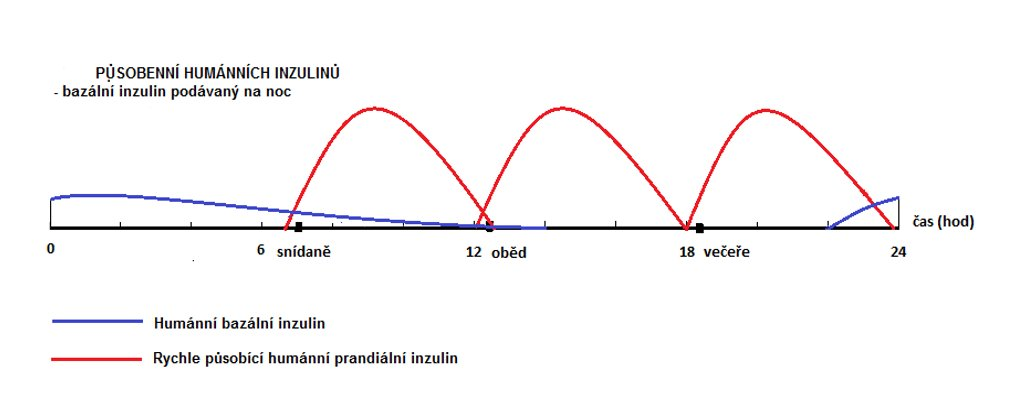
\includegraphics[width=1\textwidth]{img/pusobeni-humannich-inzulinu.jpg}
\textit{Zdroj: www.cukrovka.cz}
\end{figure}

Další možností je postupné dávkování inzulinu v malých dávkách během celého dne pomocí inzulinové pumpy (viz kapitola \ref{ch:pumpa}).


\subsection{Inzulinová pumpa}
\label{ch:pumpa}

Inzulin se podává injekčně do podkoží. Jednou z možností jsou inzulinová pera (aktuálně nejrozšířenější způsob podání inzulinu). Jedná se o lepší variantu klasické injekční stříkačky schopné dávkovat inzulin s přesností na 0,5 jednotky inzulinu.

Další možností aplikace inzulinu je inzulinová pumpa. Ta umožňuje kontinuální podání bazální dávky rychle působícího inzulinu. Simuluje tak reálnou funkci zdravé slinivky, která by za normálních okolností produkovala malé množství inzulinu pro udržení glykémie. Příjem jídla se vykreje nastavením požadovaného bolusu.

Na některých pumpách lze nastavit více bazálních dávek inzulinu přizpůsobených režimu daného dne (například víkendové aktivity nebo sport). Některé lze také propojit se systémem kontinuální monitorace glukózy, viz kapitola \ref{ch:monitorace}. \cite{Diabetes.Perusicova,Diabetes.Rybka} 


\section{Monitorace glukózy}
\label{ch:monitorace}

Monitoring je důležitý pro správné určení léčby, které provádí diabetolog.

Součástí monitorace je měření koncentrace glukózy a ketolátek v krvi a moči. Dále se kontroluje krevní tlak, hmotnost (BMI). Zaznamenávat by se měli denní dávky inzulinu, příjem karbohydrátů, hypo- a hyperglykémie a situace vyžadující úpravu dávkování inzulinu jako je zvýšená fyzická aktivita nebo nemoc. Při pravidelné kontrole u lékaře se vyšetřuje množství glykovaného hemoglobinu, cholesterolu, činnost ledvin a neuropatie.

Frekvence monitoringu je individuální a závislá na mnoha faktorech a potřebách daného pacienta. Selfmonitoring by se měl provádět denně před aplikací inzulinu, zhruba 3-4x denně, v noci v případě rizika hypoglykémie a v době nástupu dawn fenoménu (ranní hyperglykémie). Výsledek běžného denního měření se nazývá malý glykemický profil. Častější monitoring je třeba v případě zvláštních situací vyžadujících úpravu dávkování inzulinu a v těhotenství. Takové měření se nazývá malý glykemický profil.

Nejčastěji se glykémie měří glukometrem z kapky krve nanesené na diagnostický proužek. Tato metoda, která zahrnuje vpich do konečku prstu může být pro pacienta bolestivá a odradit ho od častějších měření. \cite{Diabetes.Pelikan}

\subsection{CGMS}

Alternativou k jednorázovým měřením je kontinuální monitorace glukózy (CGMS - Continuous Glucose Monitoring System). Pro měření se zavede elektrochemický glukózový senzor do podkoží, kde se měří koncentrace glukózy v plazmě v intersticiální (mezibuněčné) tekutině. Tento systém umožňuje měření hladiny glukózy po celý den v minutových nebo pětiminutových intervalech (na českém trhu jsou dostupné přístroje měřící v pětiminutových intervalech). To umožňuje sledovat vývoj glykémie během dne.

Hodnoty ze senzoru a hodnoty naměřené z krve se mohou lišit, protože měření probíhá v intersticiální tekutině, kam se glukóza dostává z krve s menším zpožděním, jsou naměřené hodnoty také se zpožděním vůči reálné hodnotě v krvi. Také v některých případech jsou koncentrace v intersticiální tekutině nižší než v krvi, zejména v noci. Senzor se také musí pro správnou funkci denně kalibrovat (alespoň 2x) hodnotami naměřenými z krve při stabilní glykémii. \citep{Diabetes.Perusicova}

Přístroje disponují alarmem signalizujícím vzestup či pokles glykémie. Do CGMS se zadává také množství přijatých karbohydrátů z jídla a fyzická aktivita. Z dat CGMS pak lze lépe určit vývoj glykémie v závislosti na daných aktivitách.

Některé přístroje umožňují integraci s kompatibilní inzulinovou pumpou a zadání požadované bazální hladiny inzulinu a bolusů. Aktuální hybridní systémy jsou schopny upravovat hladinu bazálu podle naměřených hodnot. Takovým systémem je například systém OpenAPS, který ale není oficiálně schválený jako zdravotnický prostředek a tudíž není zaručena jeho správná funkcionalita. Plně autonomní systém ale zatím neexistuje. Je to z důvodu, že hladinu glukózy ovlivňuje mnoho faktorů, které přístroje na trhu nejsou schopny spolehlivě rozeznat. Jedná se především o rychlé zvýšení glykémie po jídle a podání odpovídajícího bolusu. Ten je navíc doporučen aplikovat půl hodiny před jídlem.

Rizikem autonomních systémů je podání příliš velkého množství inzulinu a stavu hypoglykémie, která je mnohonásobně horší než riziko hyperglykémie. Řešením by mohl být dávkovač glukagonu, který by při poklesu glykémie hladinu opět vyrovnal. \citep{cukrovka.cz}

\chapter{Analýza metod detekce příjmu karbohydrátů}
\addtocontents{toc}{\protect\setcounter{tocdepth}{1}}

Detekce příjmu karbohydrátů je důležitou součástí autonomních systémů CGMS a inzulinové pumpy. Při příjmu karbohydrátů se zvyšuje koncentrace glukózy v krvi, kterou je nutno korigovat bolusem inzulinu, aby se předešlo stavu hyperglykémie. Tato dávka inzulinu musí odpovídat množství přijatých karbohydrátů. Příliš velká dávka může vést k hypoglykémii.

Metody detekce karbohydrátů mohou být model-based nebo data-driven.

Většina studií je založená na implementaci fyzického modelu (většinou Bergmanův minimální model) a aplikaci predikčního algoritmu, jako je například Kalmanův filtr pro predikci jednotlivých stavů (glykémie a karbohydráty). Detekce karbohydrátů je pak porovnáním pozorovaných stavů a modelu vůči definovanému thresholdu, výpočtu cross-covariance nebo aplikováním rozhodovacích pravidel.

U data-driven metod se vychází z naměřených dat. Extrakce vlastností je u těchto metod kvantitativní nebo kvalitativní. Kvantitativní metoda je například analýza hlavních komponent. V kvalitativních modelech jsou časová data převedena na sekvenci kvalitativních proměnných k vytvoření kvalitativní reprezentace dat. Data-driven metody jsou méně závislé na přesnosti fyzického modelu, ale je potřeba pro jejich natrénování velkého množství vzorků. Mezi data-driven metody patří i neuronové sítě.

\section{Bergmanův minimální model}

Bergmanův minimální model \citep{analyzaCHO.Bergman} je nelineární dynamický model koncentrace glukózy v plazmě. Tento model popisuje vývoj hladiny glukózy v plazmě na základě koncentrace a účinnosti inzulinu a přijatých karbohydrátů. Model určuje sada diferenciálních rovnic prvního řádu:

$\frac{dF(t)}{dt}=-p_{1}G(t)-p_{4}I_{eff}(t)G(t)+p_{1}G_{b}+R_{a}(t)$

$\frac{dI_{eff}(t)}{dt}=-p_{2}I_{eff}(t)+p_{3}I_{p}(t)$

\noindent kde $G_b$ je koncentrace glukózy v plazmě, $I_p$ je koncentrace inzulinu v plazmě, $I_eff$ je koncentrace efektivního inzulinu, $p_1, p_2, p_3, p_4$ jsou parametry a $R_a (t)$ je míra výskytu glukózy definovaná jako:

\scalebox{1.2}{$R_{a}(t)=\frac{C(t)}{V\tau^{2}}te^{-\frac{t}{\tau}}$}

\noindent kde $C(t)$ je množství přijatých karbohydrátů, $V$  je distribuční objem a $\tau$ je vrchol absorbce karbohydrátů \citep{analyzaCHO.Turksoy}.


\section{Model-based metody}
\subsection{Real-time insulin bolusing for unannounced meals with artificial pancreas}
\label{ch:analyzaCHO:turksoy}

Pro detekční algoritmus této metody použili \citet{analyzaCHO.Turksoy} upravený Bergmanův minimální model. Unscented Kalmanův filtr je použit pro odhad stavů a parametrů minimálního modelu.

Model definuje rychlost výskytu glukózy \textbf{Ra(t)} na základě množství přijatých karbohydrátů C(t), distribučního objemu V a maximální doby absorbce jídla \textit{tau}:

\scalebox{1.2}{$R_{a}(t)=\frac{C(t)}{V\tau^{2}}te^{-\frac{t}{\tau}}$}

Rychlost výskytu glukózy \textbf{Ra(t)} je použita pro výpočet příjmu karbohydrátů. Bolus karbohydrátů je detekován pokud Ra(t) je větší než 2 mg/dl/min a naměřená hodnota z CGM je větší než 100mg/dl. Další příjem karbohydrátů může být detekován až když Ra(t) klesne pod hranici 2 mg/dl/min a uplyne alespoň 30 minut od posledního bolusu.

Testování bylo provedeno na sedmi reálných pacientech, kdy v první části experimentu si pacient aplikoval inzulin sám na základě doporučení diabetologa a ve druhé části bylo dávkování inzulinu řízeno algoritmem pro detekci karbohydrátů. Nutno podotknout, že experimentu se zúčastnili mladí lidé s optimálním glykemickým profilem.

Na obrázku \ref{fig:turksoy2} je porovnání obou způsobů. Experiment ukázal, že výsledky jsou statisticky ekvivaletní (hladina významnosti p=0.05).

\begin{figure}[H]
\caption{Porovnání řízení aplikace inzulinu pacientem a algoritmem pro detekci karbohydrátů}
\label{fig:turksoy2}
\centering
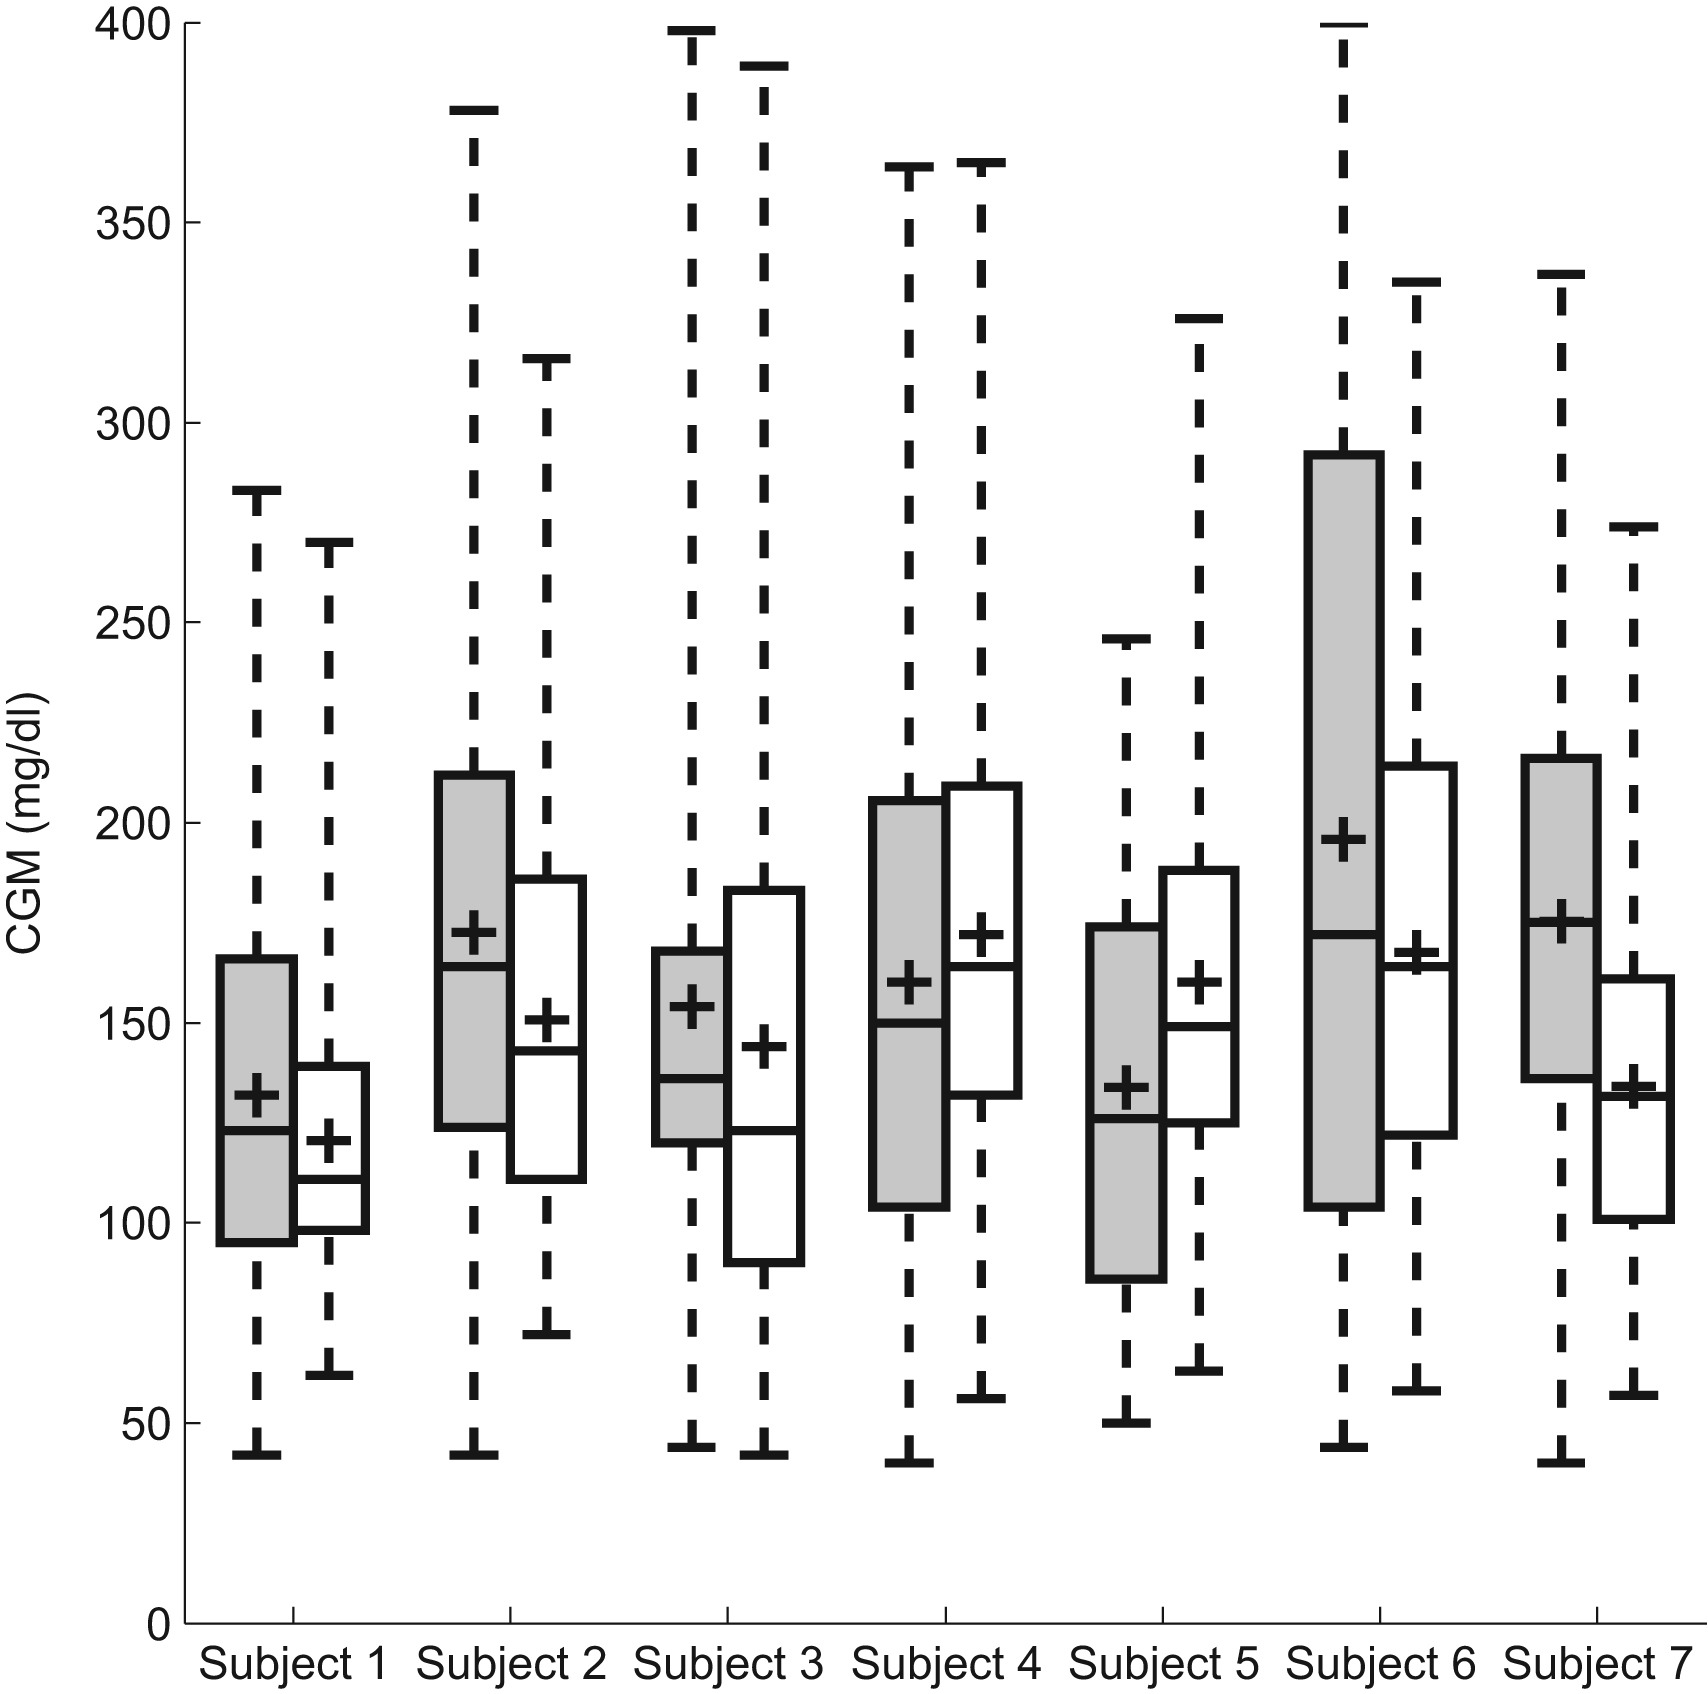
\includegraphics[width=0.8\textwidth]{img/analyzaCHO/turksoy3.jpg}\\
\textit{Zdroj: Real-time insulin bolusing for unannounced meals with artificial pancreas \citep{analyzaCHO.Turksoy}}
\end{figure}


\subsection{Unannounced Meals in the Artificial Pancreas: Detection Using Continuous Glucose Monitoring}
\label{ch:analyzaCHO:CrossCovariance}

Autoři \citet{analyzaCHO.CrossCovariance} počítají cross-covarianci mezi naměřenými hodnotami glukózy a jejich odhadem dopředného rozdílu chybového parametru $D_{diff}$ (Unscended Kalman filter) přes tři posuvná časová okna. Pro každé okno je aplikován jiný threshold pro detekci, přičemž se snižuje riziko falešně pozitivní detekce.

\begin{figure}[H]
\caption{Naměřené hodnoty glukózy (graf 1), cross-covariance (graf 2), $D_{diff}$ parameter (graf 3)}
\label{fig:analyza:crosscovariance1}
\centering
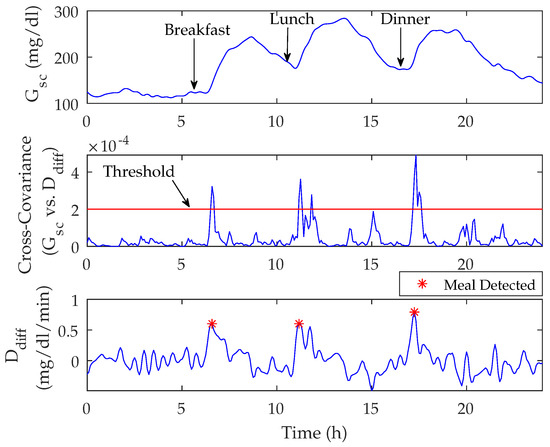
\includegraphics[width=0.8\textwidth]{img/analyzaCHO/crosscovariance1.jpg}\\
\textit{Zdroj: Unannounced Meals in the Artificial Pancreas: Detection Using Continuous Glucose Monitoring \citep{analyzaCHO.CrossCovariance}}
\end{figure}

Úspěšnost detekce jednotlivých oken je v tabulce na obrázku \ref{fig:analyza:crosscovariance2}, zpoždění detekce vzhledem k množství přijatých karbohydrátů v tabulce na obrázku \ref{fig:analyza:crosscovariance3}.

\begin{figure}[H]
\caption{Úspěšnost detekce}
\label{fig:analyza:crosscovariance2}
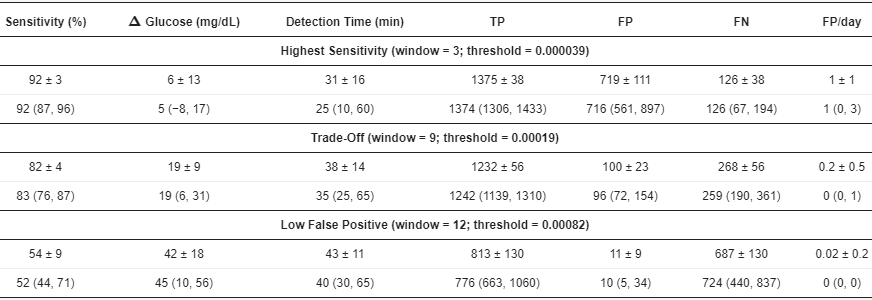
\includegraphics[width=1\textwidth]{img/analyzaCHO/crosscovariance2.png}\\
\textit{Zdroj: Unannounced Meals in the Artificial Pancreas: Detection Using Continuous Glucose Monitoring \citep{analyzaCHO.CrossCovariance}}
\end{figure}

\begin{figure}[H]
\caption{Zpoždění detekce}
\label{fig:analyza:crosscovariance3}
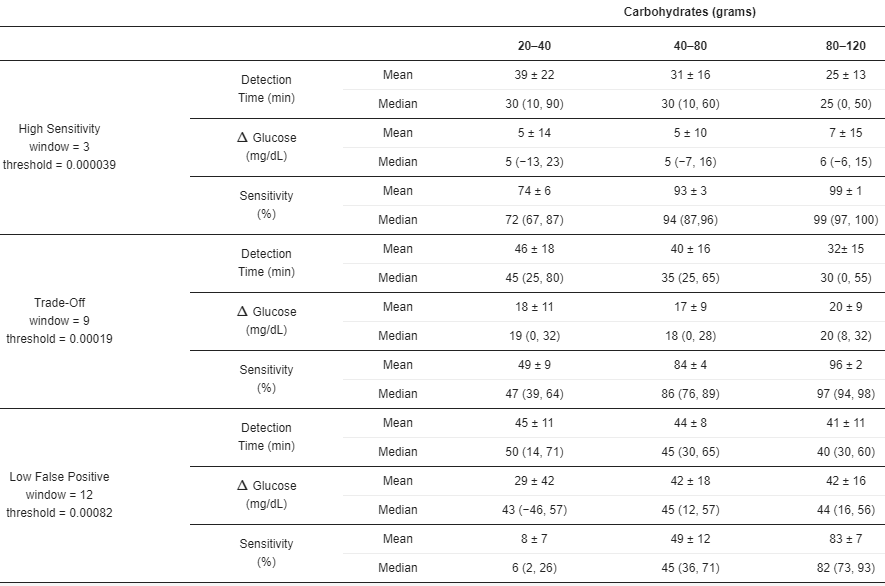
\includegraphics[width=1\textwidth]{img/analyzaCHO/crosscovariance3.png}\\
\textit{Zdroj: Unannounced Meals in the Artificial Pancreas: Detection Using Continuous Glucose Monitoring \citep{analyzaCHO.CrossCovariance}}
\end{figure}


\subsection{Probabilistic Evolving Meal Detection and Estimation of Meal Total Glucose Appearance}
\label{ch:analyzaCHO:diff}

V této práci \citet{analyzaCHO.Diff} použili inzulino-glukózový model, který udává rychlost změny intersticiální glukózy závislé na působení inzulínu a endogenní produkci glukózy. Provede se analýza změn rozdílů mezi modelovanou rychlostí změny intersticiální glukózy a naměřenou CGM. Následně jsou navzorkovány experimentálně zjištěná data příjmu karbohydrátů od 0~g do 100~g (10 vzorků) a na základě pravděpodobnosti se určí nejlepší odhad.

Na obrázku \ref{fig:analyza:diff1} je znázorněn provedený experiment při příjmu 0,33~g a 69~g karbohydrátů. První graf znázorňuje rozdíl mezi předpokládanou modelovou hodnotou glukózy a naměřenou hodnotou. Prostřední graf ukazuje pravděpodobnost příjmu karbohydrátů. Spodní graf ukazuje odhadovaný celkový výskyt glukózy z přijatého jídla. Hranice pro detekci je pravděpodobnost 10 \%.

\begin{figure}[H]
\caption{Detekce karbohydrátů v čase}
\label{fig:analyza:diff1}
\centering
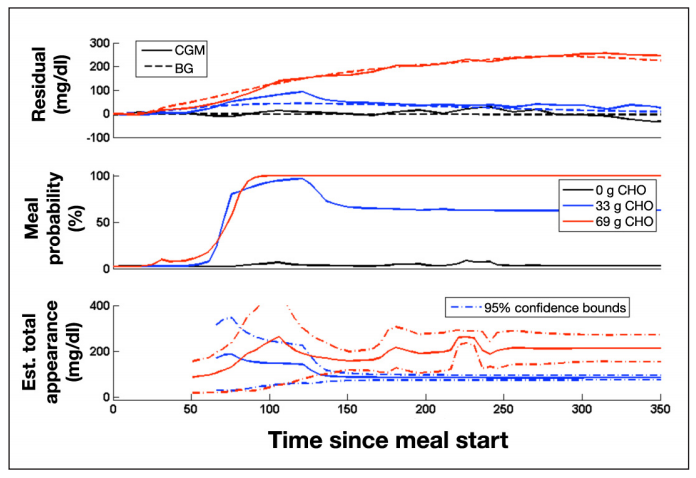
\includegraphics[width=0.8\textwidth]{img/analyzaCHO/diff1.png}\\
\textit{Zdroj: Probabilistic Evolving Meal Detection and Estimation of Meal Total Glucose Appearance \citep{analyzaCHO.Diff}}
\end{figure}

Experiment byl proveden pro 99 scénářů. Pro 11 scénářů bez jídla nebyly žádné falešně pozitivní detekce. Pro scénáře, kdy byly přijaté karbohydráty, byl algoritmus úspěšný podle množství přijatých karbohydrátů, jak je vidět na obrázku \ref{fig:analyza:diff2}.

\begin{figure}[H]
\caption{Úspěšnost detekce vzhledem hladině glukózy a množství přijatých karbohydrátů}
\label{fig:analyza:diff2}
\centering
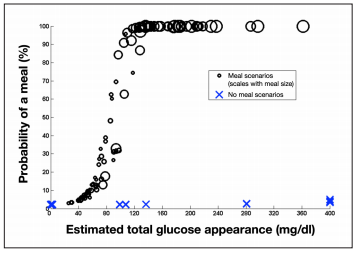
\includegraphics[width=0.8\textwidth]{img/analyzaCHO/diff2.png}\\
\textit{Zdroj: Probabilistic Evolving Meal Detection and Estimation of Meal Total Glucose Appearance \citep{analyzaCHO.Diff}}
\end{figure}


\subsection{An Unannounced Meal Detection Module for Artificial Pancreas Control Systems}
\label{ch:analyzaCHO:nekonzistence}

\citet{analyzaCHO.Nekonzistence} navrhli metodu, která využívá lineárního Kalmanova filtru nad linearizovaným Bergmanovým modelem. Přijaté karbohydráty pak způsobují nekonzistentnost tohoto filtru. Jak je v práci podotknuto, lineární Kalmanův filtr není pro tuto úlohu ideální vzhledem k tomu, že glykoregulační systém diabetického pacienta je nelineární a hladina glukózy může během dne kolísat i bez zjevných příčin. Proto se v jiných pracích používá nelineární Unscented Kalmanův filtr. Úspěšnost a rychlost detekce pro různou velikost jídel je vidět v tabulce na obrázku \ref{fig:analyza:nekonzistence}.

\begin{figure}[H]
\caption{Úspěšnost detekce vzhledem hladině glukózy a množství přijatých karbohydrátů}
\label{fig:analyza:nekonzistence}
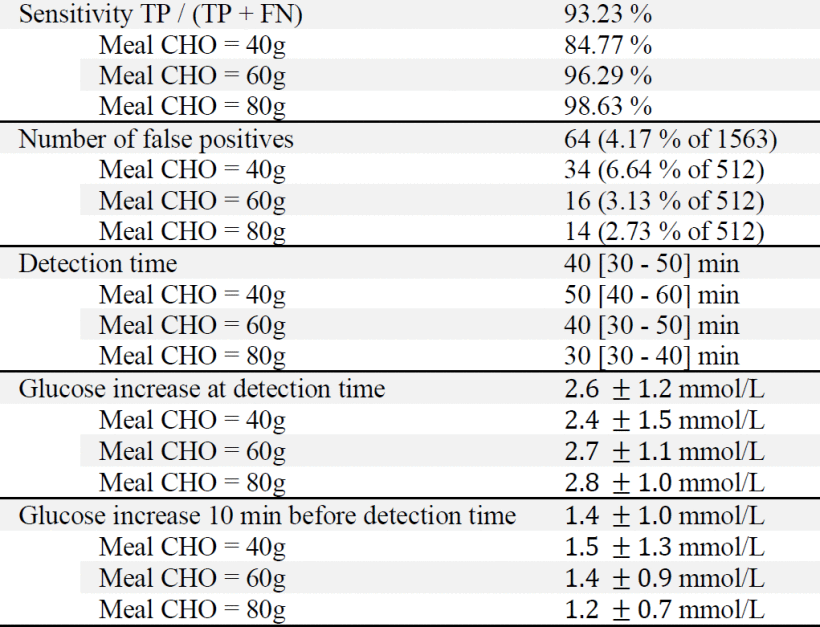
\includegraphics[width=1\textwidth]{img/analyzaCHO/nekonzistence.png}\\
\textit{Zdroj: An Unannounced Meal Detection Module for Artificial Pancreas Control Systems \citep{analyzaCHO.Nekonzistence}}
\end{figure}


\subsection{Committed Moving Horizon Estimation for Meal Detection and Estimation in Type 1 Diabetes}
\label{ch:analyzaCHO:horizon}

Committed Moving Horizon Estimation (CMHE) \citep{analyzaCHO.MovingHorizon} umožňuje predikovat čas a velikost nehlášených jídel. Metoda je založena na Moving Horizon Estimation (MHE). MHE je metoda odhadů omezených stavů nelineárního diskrétního modelu, která predikuje sekvenci stavových proměnných a poruch $\delta$ (disturbance) tak, že minimalizuje chybu mezi predikovanými a měřenými hodnotami \citep{analyzaCHO.MovingHorizon}. V případě detekce karbohydrátů je modelem glukózo regulační systém člověka (ve studii je použit Bergmanův minimální model) a poruchami se rozumí přijaté karbohydráty. MHE, na rozdíl od Kalmanova filtru, nepočítá s normálním rozdělením poruch. 

Pro každou instanci MHE (časové okno velikosti N) je N odhadů disturbance hodnoty (pro t až t-N). V každém časovém bodě t tak máme N odhadů v čase t+N. Problémem je, který z N odhadů vybrat. Prvotní odhad v čase t není přesný, protože tento odhad zohledňuje pouze naměřené hodnoty před časem t, zatímco zvýšení hladiny glukózy se projeví až s časovým odstupem od přijetí karbohydrátů v závislosti na metabolismu daného člověka. Odhad v čase t+N zase nezohledňuje vývoj glukózy v minulosti a zároveň je k dispozici s velkým zpožděním. Tento problém řeší CMHE, který nebere jednu disturbance hodnotu, ale kompromis mezi predikovanými a naměřenými hodnotami. Výsledná hodnota disturbance parametru v čase $\Delta_{t-V}$ je vypočítá jako vážený průměr odhadů v daný čas z předchozích iterací včetně (obrázek \ref{fig:analyza:horizon1}):

\scalebox{1.5}{$\Delta_{t-V}=\frac{(\sum^{t}_{i=t-V+1}W(i)^{b}\cdot \delta^{i}_{t-V})}{\sum^{t}_{i=t-V+1}W(i)^{b}}$}

kdy V je commitment level, V<N, $\delta$ je disturbance parametr, W(i) jsou váhy prioritizující odhady mezi predikovanými a naměřenými hodnotami.

\begin{figure}[H]
\caption{Disturbance paremetr $\delta$ několik časových oken}
\label{fig:analyza:horizon1}
\centering
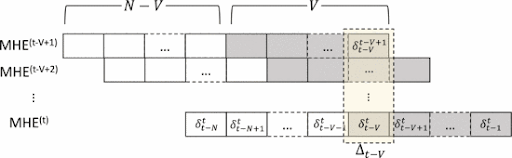
\includegraphics[width=1\textwidth]{img/analyzaCHO/horizon1.png}\\
\textit{Zdroj: Committed Moving Horizon Estimation for Meal Detection and Estimation in Type 1 Diabetes \citep{analyzaCHO.MovingHorizon}}
\end{figure}

CMHE instance (min Ct) se optimalizují pomocí Mixed-integer Quadratic Programming (MIQP), který disturbance parametr reprezentuje jako čtvercovou vlnu (za předpokladu, že příjem karbohydrátů po dobu jídla je konstantní). Jídlo je detekováno pokud $\Delta t$ je nad daným thresholdem alespoň 80 \% času w.

V provedeném experimentu je měření prováděno každou minutu, časové okno N = 180, commitment level V = 40, w = 5 minut. Na obrázku \ref{fig:analyza:horizon4} je srovnání MHE a CMHE v závislosti na nastaveném thresholdu.  V tabulce \ref{tab:analyza:horizon5} jsou výsledky experimentu pro optimálně nastavený threshold (černý trojúhelník). Metoda dosahuje 100 \% úspěšnost detekce pro hlavní jídla, celkových 88.5 \% je způsobeno menšími jídly, pro jejichž lepší detekci by musel být snížen threshold. To by ale vedlo ke zvýšení falešných detekcí, kterých je v průměru 2.6 za den. Průměrná doba detekce je 20 minut \citep{analyzaCHO.MovingHorizon}.

\begin{figure}[H]
\caption{Detekce MHE (modrá) a CMHE (červená)}
\label{fig:analyza:horizon4}
\centering
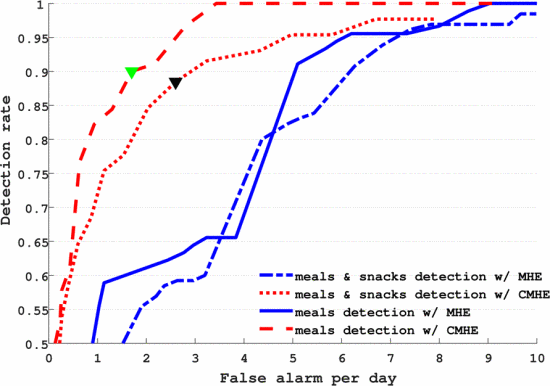
\includegraphics[width=0.9\textwidth]{img/analyzaCHO/horizon4.png}\\
\textit{Zdroj: Committed Moving Horizon Estimation for Meal Detection and Estimation in Type 1 Diabetes \citep{analyzaCHO.MovingHorizon}}
\end{figure}

\begin{table}[H]
\caption{Výsledky}
\label{tab:analyza:horizon5}
\centering
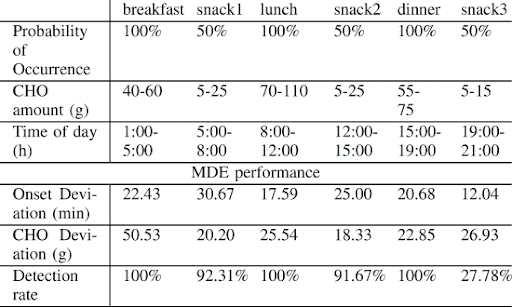
\includegraphics[width=1\textwidth]{img/analyzaCHO/horizon5.png}\\
\textit{Zdroj: Committed Moving Horizon Estimation for Meal Detection and Estimation in Type 1 Diabetes \citep{analyzaCHO.MovingHorizon}}
\end{table}


\section{Data-driven metody}
\subsection{Unannounced Meal Detection for Artificial Pancreas Systems Using Extended Isolation Forest}
\label{ch:analyzaCHO:forest}

Isolation forest je metoda, která detekuje a izoluje anomálie v datech. Data jsou rekurzivně rozdělena do stromové struktury (iTree - isolation tree) náhodným výběrem atributů z daných vlastností (feature) dokud nejsou jednotlivé instance izolovány. Toto náhodné rozdělení má pro anomálie signifikantně kratší cestu ve stromové struktuře \citep{analyzaCHO.IsolationForest}.

Vlastnosti, které slouží jako vstup pro Extended isolation forest \citep{analyzaCHO.ExtendedIsolationForest} jsou derivace naměřené glukózy v plazmě \textbf{dGp}, zadané karbohydráty (pokud byly zadány) a podaný inzulin. Pro výpočet derivace glukózy v čase t \textbf{dGp(t)} je potřeba znát naměřenou glukózu v čase t+1 \textbf{Gp(t+1)}. Z toho důvodu nastává zpoždění detekce o 5 minut. Detekce anomálií je pak pomocí dvou thresholdů pro menší a větší míru rizika nezadaných karbohydrátů.
Příklad detekce anomálií je na obrázku \ref{fig:analyza:forest}. Notifikace je vznešena pokud se objeví jedna anomálie s větší mírou rizika (červené), nebo 3 anomálie s menší mírou rizika (modré).

\begin{figure}[H]
\caption{Úspěšnost detekce vzhledem hladině glukózy a množství přijatých karbohydrátů}
\label{fig:analyza:forest}
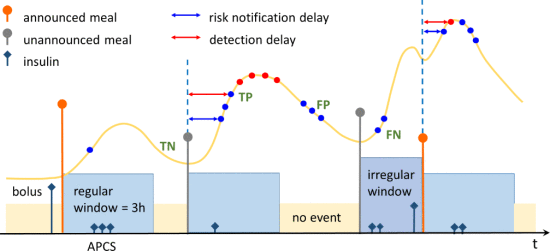
\includegraphics[width=1\textwidth]{img/analyzaCHO/forest.png}\\
\textit{Zdroj: Unannounced Meal Detection for Artificial Pancreas Systems Using Extended Isolation Forest \citep{analyzaCHO.ExtendedIsolationForest}}
\end{figure}

Metoda byla testována na čtyřech virtuálních pacientech (pro jejich simulaci byl využit Hovorkovo model) V simulovaných pětidenních denních scénářích přijal pacient průměrně 3,4 jídla za den. Pro scénář, kdy bylo jídlo v 50 \% zadáno a v 50 \% nezadáno, dosahovala metoda úspěšnosti 90,8 \% a v 6,2 \% případů byla falešně pozitivní. V případě, že jídlo nebylo zadáno vůbec, byla úspěšnost 90,0 \% a v 11,47 \% falešně pozitivní. Zpoždění detekce je 26-39 minut \citep{analyzaCHO.ExtendedIsolationForest}.


\subsection{A Closed-Loop Artificial Pancreas Using Model Predictive Control and a Sliding Meal Size Estimator}
\label{ch:analyzaCHO:thrashold}

\citet{analyzaCHO.Thresholds} použili hlasovací schéma pro detekci karbohydrátů. Algoritmus je založen na kontinuálním  pozorování první a druhé derivace koncentrace glukózy, které při splnění kritérii vyšle sérii impulsů (až 15 impulsů během 30ti minut). Tato metoda je založena na vzorkování po jedné minutě.

Impulsy jsou vyslány při překročení thresholdu. Pro nastavení thresholdu se vychází z toho, že jedno jídlo způsobí nárůst rychlosti výskytu glukózy v krvi $dG$ (první derivace) 0-2 mg/dl/min, druhé derivace $d_{2}G$ 0-0,02 mg/dl/min2. Thresholdy jsou proto nastaveny na {0, 0.5, 1.25, 1.8} pro $dG$ a {0, 0.005, 0.0125, 0.018} pro $d_{2}G$. Jelikož je mezi $dG$ a $d_{2}G$ zpoždění, další impuls je vyslán pokud se hodnoty kříží. Vyslání impulsů je na obrázku \ref{fig:analyza:threshold1}.
 
Tyto impulsy jsou poté zesíleny a převedeny na gramy karbohydrátů (ve studii počítají se 4~g na impuls), viz obrázek \ref{fig:analyza:threshold2}.

Počet impulsů, časové okno, thresholdy a množství karbohydrátů na impuls lze individuálně změnit podle diabetického profilu pacienta.

\begin{figure}[H]
\caption{Impulsy}
\label{fig:analyza:threshold1}
\centering
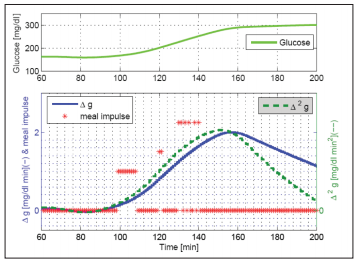
\includegraphics[width=0.8\textwidth]{img/analyzaCHO/threshold1.png}\\
\textit{Zdroj: A Closed-Loop Artificial Pancreas Using Model Predictive Control and a Sliding Meal Size Estimator \citep{analyzaCHO.Thresholds}}
\end{figure}
\begin{figure}[H]
\caption{Predikované karbohydráty}
\label{fig:analyza:threshold2}
\centering
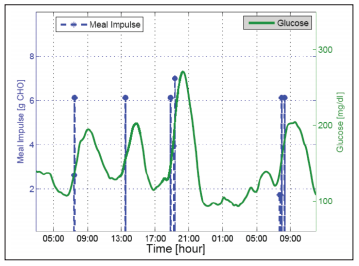
\includegraphics[width=0.8\textwidth]{img/analyzaCHO/threshold2.png}\\
\textit{Zdroj: A Closed-Loop Artificial Pancreas Using Model Predictive Control and a Sliding Meal Size Estimator \citep{analyzaCHO.Thresholds}}
\end{figure}

V tabulce \ref{tab:analyza:threshold3} jsou uvedeny výsledky provedeného testování. Algoritmus dosahuje úspěšnost 82 \% a průměrný odhad jídla je 36,41~g karbohydrátů. Zpoždění detekce je průměrně 31 minut \citep{analyzaCHO.Thresholds}.

\begin{table}[H]
\caption{Výsledky}
\label{tab:analyza:threshold3}
\centering
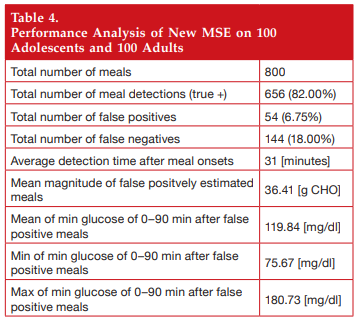
\includegraphics[width=0.8\textwidth]{img/analyzaCHO/threshold3.png}\\
\textit{Zdroj: A Closed-Loop Artificial Pancreas Using Model Predictive Control and a Sliding Meal Size Estimator \citep{analyzaCHO.Thresholds}}
\end{table}


\subsection{Meal Detection and Carbohydrate Estimation Using Continuous Glucose Sensor Data}
\label{ch:analyzaCHO:wavelet}

V této studii \citet{analyzaCHO.WaveletEst} použili waveletové filtrování pro odstranění šumu z dat naměřených CGM. Waveletové filtrování rozdělí frekvenční obsah vstupních dat do několika pásem, kde se jinou měrou projevuje šum a užitečná složka \citep{analyzaCHO.Wavelet}. Zvolený parametr míry filtrování musí být dostatečně velký, aby odfiltroval šum, ale ne přiliš, aby se neodfiltrovaly ostré nárůsty způsobené příjmem karbohydrátů.

Pro extrakci vlastností je použita trojúhelníková kvalitativní reprezentace. V kvalitativních metodách extrakce dat jsou časová data konvertována na sekvenci kvalitativních proměnných. Pro trojúhelníkovou kvalitativní reprezentaci jsou kvalitativní proměnné trojúhelníky (viz obrázek \ref{fig:analyza:wavelet1}). Trojúhelníky dělí data na epizody (obrázek \ref{fig:analyza:wavelet2}) jejichž hraniční body jsou buďto extrém ($dG/dt=0$) nebo inflexní bod ($d_{2}G/dt=0$). Epizody se nepřekrývají a každé dvě sousední jsou rozdílné. Hodnoty dx a ddx jsou vypočteny z numerické derivace a mapovány na +/0/-.

\begin{figure}[H]
\caption{Kvalitativní proměnné trojúhelníkové kvalitativní reprezentace}
\label{fig:analyza:wavelet1}
\centering
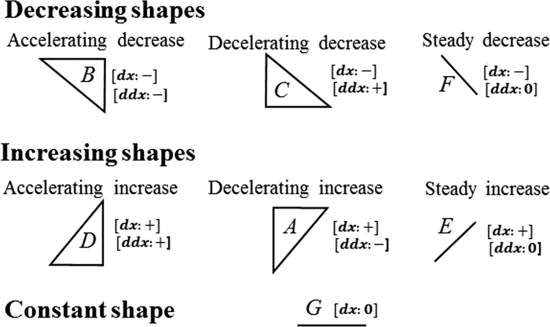
\includegraphics[width=0.8\textwidth]{img/analyzaCHO/wavelet1.png}\\
\textit{Zdroj: Meal Detection and Carbohydrate Estimation Using Continuous Glucose Sensor Data \citep{analyzaCHO.WaveletEst}}
\end{figure}
\begin{figure}[H]
\caption{Data rozdělená na epizody}
\label{fig:analyza:wavelet2}
\centering
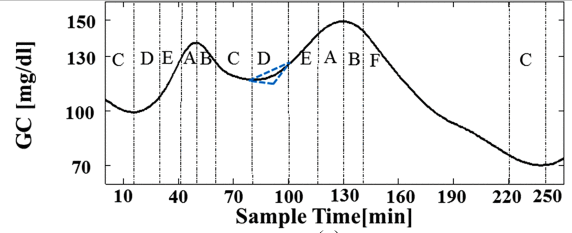
\includegraphics[width=0.8\textwidth]{img/analyzaCHO/wavelet2.png}\\
\textit{Zdroj: Meal Detection and Carbohydrate Estimation Using Continuous Glucose Sensor Data \citep{analyzaCHO.WaveletEst}}
\end{figure}

Pro tuto studii byla definice epizod modifikována tak, že velikost epizody je pevně dána a obsahuje určitý počet vzorků. Epizody se překrývají a sousední mohou být stejné. Výpočet dx a ddx udávající tvar trojúhelníku je:

$d^{1}G(n)=G(n)-G(n-l_{e})$

$d^{2}G(n)=G'(n)-G'(n-l_{e})$

$G'(n)=G(n)-G(n-1)$

Do trojúhelníkové reprezentace se přidá neurčitost (fuzzy logika) tak, že epizodu popisuje více tvarů trojúhelníků (definují se další způsoby pro výpočet $d^1x$ a $d^2x$).

Pro detekci příjmu karbohydrátů se každému trojúhelníku přiřadí váha odpovídající tvaru. Vynásobením vah s vektorem fuzzy trojúhelníkové reprezentace vznikne proměnná \textit{“increase of glucose trend index”} Igt pro každý vzorek (váhy jsou nastaveny tak, že hodnota $I_gt$ je v intervalu<-3;3>). Pakliže hodnota Igt (nebo součet Igt v časovém okně) překročí hranici 2,5, je detekován příjem.

Úspěšnost detekce byla u dospělých 87 \% (falešně pozitivní 21 \%) a u dětí 93 \% (falešně pozitivní 3 \%). Zpoždění detekce je přibližně půl hodiny \citep{analyzaCHO.WaveletEst}.


\subsection{Pattern Recognition Reveals Characteristic Postprandial Glucose Changes: Non-Individualized Meal Detection in Diabetes Mellitus Type 1}
\label{ch:analyzaCHO:lda}

\citet{analyzaCHO.LDA} použili Moving horizon estimator pro odhad glukózy a lineární diskriminační analýzu pro klasifikaci.

Porovnávány jsou 4 metody (2 na základě klasifikace a 2 metody pro porovnání za použití thresholdu):

\begin{enumerate}
\item \textbf{Klasifikace odhadu Ra horizontů} \\
Odhady rychlosti výskytu glukózy Ra horizontů jsou predikovány na základě Bergmanova modelu. Na tyto Ra je použita Lineární diskriminační analýza (LDA).
\item \textbf{Klasifikace CGM horizontů} \\
Klasifikace je na hrubých vyhlazených datech z CGM modulu. Také v tomto případě je použita LDA.
\item \textbf{Threshold pro aktuální Ra odha} \\
Detekce přijatých karbohydrátů je pokud Ra překročí daný threshold (viz kapitola \ref{ch:analyzaCHO:turksoy}).
\item \textbf{GRID algoritmus} \\
Threshold pro naměřené hodnoty glukózy a jejich rychlost změny.
\end{enumerate}

Na obrázku \ref{fig:analyza:lda1} je výkonnost jednotlivých metod při provedeném experimentu. Je vidět, že metody využívající LDA si vedly výrazně lépe. Jejich úspěšnost se pohybuje kolem 88 \%. Také v případě času potřebného k detekci překonaly metody založené na thresholdu. Srovnání zpoždění u jednotlivých metod je na obrázku \ref{fig:analyza:lda2}.

\begin{figure}[H]
\caption{Úspěšnost detekce jednotlivých metod}
\label{fig:analyza:lda1}
\centering
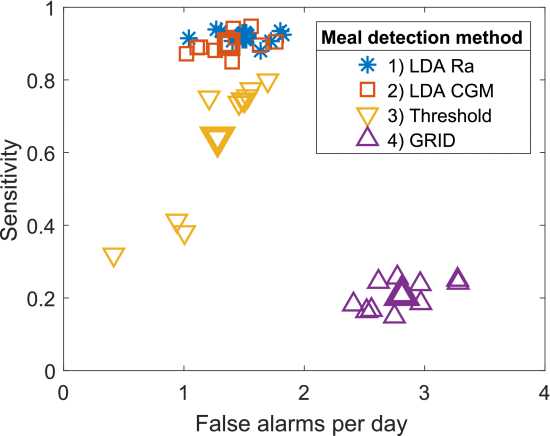
\includegraphics[width=0.6\textwidth]{img/analyzaCHO/lda1.png}\\
\textit{Zdroj: Pattern Recognition Reveals Characteristic Postprandial Glucose Changes: Non-Individualized Meal Detection in Diabetes Mellitus Type 1 \citep{analyzaCHO.LDA}}
\end{figure}
\begin{figure}[H]
\caption{Zpoždění detekce}
\label{fig:analyza:lda2}
\centering
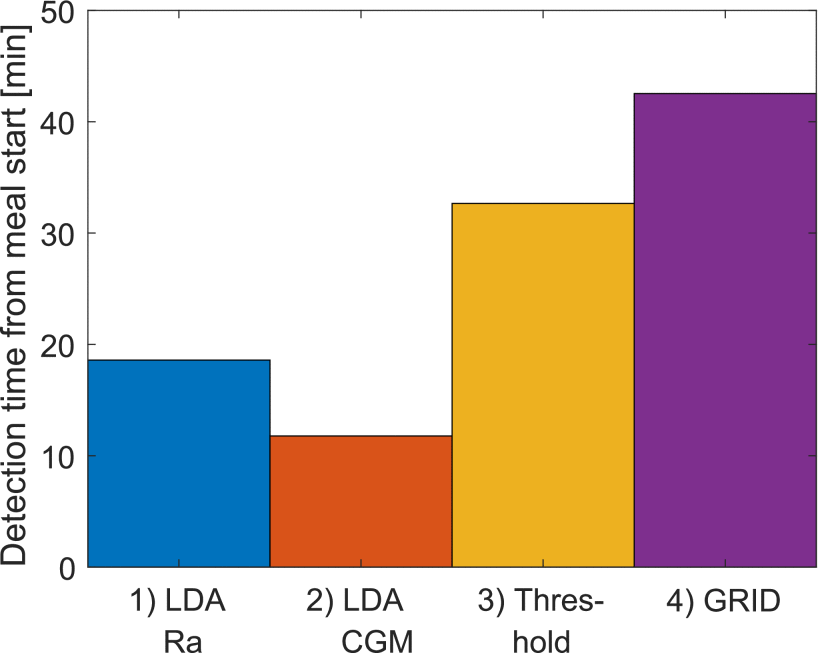
\includegraphics[width=0.6\textwidth]{img/analyzaCHO/lda2.png}\\
\textit{Zdroj: Pattern Recognition Reveals Characteristic Postprandial Glucose Changes: Non-Individualized Meal Detection in Diabetes Mellitus Type 1 \citep{analyzaCHO.LDA}}
\end{figure}


\section{Metody využívající neuronové sítě}
\subsection{Predicting the meal macronutrient composition from continuous glucose monitors}
\label{ch:analyzaCHO:neuronka}

V této studii \citet{analyzaCHO.Neuronka} použili multitaskovou neurální síť pro určení složení (karbohydráty, proteiny, tuky) v přijatém jídle.

Pro zachycení charakteristických vlastností z dat CGM byl vypočten určitý integrál (oblast pod křivkou) pro 5 časových bodů (klidový stav nalačno, zvýšená glykémie, střední hodnota při návratu do klidového stavu, pokles glukózy a konečný stav).

Multitasková neuronová síť obsahuje jednu společnou vrstvu pro vstup (vypočítané integrály) a výstupní vrstvu (viz obrázek \ref{fig:analyza:neuronka}). Aktivační funkce pro vstupní vrstvu je Rectified Linear Units (ReLU), pro výstupní lineární funkce, ztrátová funkce je Huberova ztrátová funkce. Trénování neuronové sítě bylo na 1000 epochách.

\begin{figure}[H]
\caption{Neuronová síť}
\label{fig:analyza:neuronka}
\centering
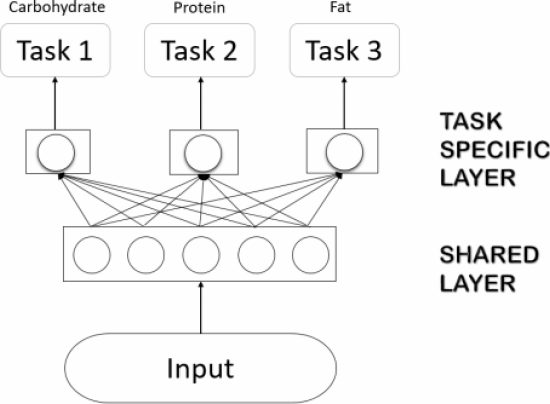
\includegraphics[width=0.7\textwidth]{img/analyzaCHO/neuronka.png}\\
\textit{Zdroj: Predicting the meal macronutrient composition from continuous glucose monitors \citep{analyzaCHO.Neuronka}}
\end{figure}

Trénování neuronové sítě a následná cross-validace byla provedena pro dva scénáře. První je natrénování neuronové sítě na datech několika pacientů a validace na datech jiného pacienta. Druhý způsob spočívá v natrénování neuronové sítě na části dat jediného pacienta (vynechání jednoho jídla) a validace na zbylých datech. Z experimentu vyšel lépe druhý způsob zohledňující metabolismus konkrétního jedince se střední kvadratickou chybou pro karbohydráty 0,39. Kvadratická chyba karbohydrátů pro první způsob je 0,45 \citep{analyzaCHO.Neuronka}. 

Metoda počítá s poměrně přesným příjmem jídla v časovém rozmezí 8 hodin. Jako vstup pro neuronovou síť pak jsou vypočtená data z tohoto celého časového okna. Při sběru dat byla také vyloučená fyzická aktivita, která ovlivňuje hladinu glukózy. Z těchto důvodů není metoda vhodná pro řízení dávkování inzulinu v reálném čase.


\subsection{Continuous glucose monitoring prediction}

V této studii \citet{analyzaCHO.LSTM} implementovali 3 různé algoritmy pro vývoj glykémie po jídle. Studie se nezabývá vlastní detekcí příjmu karbohydrátů.

Seasonal Autoregressive Integrated Moving Average (SARIMA) je regresní model pro časové řady. SARIMA počítá s trendem a sezónními parametry, které musí být před použitím nastaveny. Pro nastavení těchto parametrů byla použita autokorelace a částečná autokorelace.

V druhé metodě je použit Kalmanův filtr pro predikci vývoje hladiny glukózy pacienta.

V poslední metodě jsou implementovány dvě rekurentní neuronové sítě, konkrétně Long Short Term Memory model (LSMT). Pro druhou neuronovou síť slouží výstup LSMT jako vstup do další vrstvy spolu s konstantami. Těchto 7 konstant jsou první, druhý peak a střední hodnota Fourirovy transformace, střední hodnota a rozptyl Waveletové transformace a diskrétní Waveletové transformace provedenými nad daty CGM. Model byl natrénován na 10 epoch.

Pro výpočet chyby a ztrátové funkce u všech metod je použita střední absolutní chyba (MEA) a střední kvadratická chyba (RMSD). V tabulce \ref{tab:analyza:lstm} jsou výsledky jednotlivých metod.

\begin{table}[H]
\caption{Výsledky}
\label{tab:analyza:lstm}
\centering
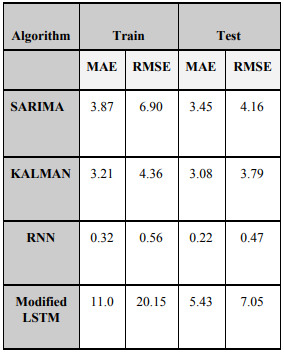
\includegraphics[width=0.6\textwidth]{img/analyzaCHO/lstm.png}\\
\textit{Zdroj: Continuous glucose monitoring prediction \citep{analyzaCHO.LSTM}}
\end{table}


\section{Porovnání jednotlivých metod}

V tabulce \ref{tab:analyza:res} je srovnání jednotlivých metod pro detekci karbohydrátů. Kritérii pro porovnání jednotlivých metod je přesnost detekce a zpoždění detekce od doby příjmu karbohydrátů.

\begin{table}[H]
\caption{Porovnání jednotlivých metod}
\label{tab:analyza:res}
\hskip-1.0cm
\begin{tabular}{|l|l|c|c|c|c|}
\hline 
\textbf{Studie} & \textbf{Zpoždění*} & \textbf{TP} & \textbf{FN} & \textbf{TN} & \textbf{FP}\tabularnewline
\hline 
\hline 
\ref{ch:analyzaCHO:turksoy} \citet{analyzaCHO.Turksoy} & - & - & - & - & -\tabularnewline
\hline 
\ref{ch:analyzaCHO:CrossCovariance} \citet{analyzaCHO.CrossCovariance} & 25-40 & 91.6\%{**} & - & - & -\tabularnewline
\hline 
\ref{ch:analyzaCHO:diff} \citet{analyzaCHO.Diff} & - & - & - & 11 & 0\tabularnewline
\hline 
\ref{ch:analyzaCHO:nekonzistence} \citet{analyzaCHO.Nekonzistence} & 30-50 & 93.23\% & 6.77\% & - & 4.17\%\tabularnewline
\hline
\ref{ch:analyzaCHO:horizon} \citet{analyzaCHO.MovingHorizon} & 20 & 88.5\% & 11.5\% & - & 2.6FP/den\tabularnewline
\hline 
\ref{ch:analyzaCHO:forest} \citet{analyzaCHO.ExtendedIsolationForest} & 26-39 & 90\% & 10\% & - & 11.47\%\tabularnewline
\hline 
\ref{ch:analyzaCHO:thrashold} \citet{analyzaCHO.Thresholds} & 31 (avg.) & 656 (82\%) & 144 (18\%) & - & 54 (6.75\%)\tabularnewline
\hline 
\ref{ch:analyzaCHO:wavelet} \citet{analyzaCHO.WaveletEst} & 30 (avg.) & 87\% & 13\% & - & 21\%\tabularnewline
\hline 
\ref{ch:analyzaCHO:lda} Ra \citet{analyzaCHO.LDA} & 18.59 & 92\% & 8\% & - & 1.5FP/den\tabularnewline
\hline 
\ref{ch:analyzaCHO:lda} CGM \citet{analyzaCHO.LDA} & 11.78 & 90\% & 10\% & - & 1.37FP/den\tabularnewline
\hline
\ref{ch:analyzaCHO:neuronka} \citet{analyzaCHO.Neuronka} & 8 hodin & 0.39{***} & & & \tabularnewline
\hline
\end{tabular}
\begin{flushleft}
* doba detekce karbohydrátů od příjetí jídla v minutách\\
{**} úspěšnost detekce jednotlivých oken v tabulce\\
{***} RMSRE - střední kvadratická chyba\\
TP - true positive\\
TN - true negative\\
FP - false positive\\
FN - false negative\\
\end{flushleft}
\end{table}


\addtocontents{toc}{\protect\setcounter{tocdepth}{2}}
\chapter{Analýza metod detekce fyzické aktivity}

Fyzická aktivita výrazně snižuje koncentraci glukózy v krvi. Z toho důvodu je potřeba před zahájením cvičení snížit dávkování inzulinu, jinak hrozí riziko hypoglykémie. Systémy kontinuální monitorace glukózy jsou sice schopny signalizovat pokles hladiny glukózy, ale tato detekce nemusí nastat včas, nebo není dostatečná. Proto je třeba detekovat parametry fyzické aktivity jako takové.

Většina publikovaných metod využívá k detekci data ze senzorů pro měření srdeční aktivity, teploty kůže, vodivosti kůže a akcelerometrů pro snímání pozice a pohybu těla. Tyto senzory mohou být externí, nebo součástí CGMS.


\section{•}

Autoři této metody využívají zařízení SenseWear® Pro Armband vyvinuté firmou BodyMedia (Pittsburgh, PA, USA). Toto zařízení je upevněno kolem ruky a sbírá data z pěti typů senzorů. Senzory snímají pozici a pohyb ruky a těla, teplotu kůže a okolí, vodivost kůže a srdeční aktivitu.
\chapter{SmartCGMS}

SmartCGMS je systém kontinuální monitorace glukózy nové generace vyvíjený na Katedře informatiky a výpočetní techniky na Fakultě aplikovaných věd Západočeské univerzity v Plzni. Umožňuje kontinuální monitoraci glukózy, modelování dynamiky glukózy a řízení inzulinové pumpy.

Aplikace je napsaná v jazyce C++ a je zkompilována pro x86-64 systémy MS Windows, macOS, Debian GNU/Linux a pro armeabi-v7a a arm64-v8a \citep{cgms.koutny}. Skládá se z filtrů, modelů, metrik a solverů.

\textbf{Filtr} je základní stavební prvek aplikace, který poskytuje určitou funkcionalitu. Ty mají jednotné rozhraní a jsou poskládány lineárně za sebou (viz příklad konfigurace na obrázku \ref{fig:scgms_filters}). To umožňuje vysokou modularitu a zaměnitelnost filtrů (například filtr, který čte data ze senzoru CGMS, se může nahradit filtrem, který přečte data uložená v logu, bez nutnosti změn ve zbytku konfigurace). Filtry spolu komunikují předáváním událostí. Událost obsahuje typ události (level, info, parameters), id filtru, který událost vytvořil, typ signálu, hodnotu, časový segment a čas vytvoření události. Nejčastější je událost typu level, která v sobě má hodnotu naměřeného nebo vypočteného signálu. Události se zpracovávají postupně tak, jak přichází. Filtr může událost poslat dál beze změny, událost upravit, nebo událost zahodit a případně vygenerovat nový signál.

Nově vytvářený filtr implementuje rozhraní \textit{scgms::IFilter} a \textit{refcnt::IReferenced}. Při vytvoření instance filtru se volá metoda \textit{Configure}, která slouží pro nastavení filtru (typicky přečtení a nastavení konfiguračních parametrů). Metoda \textit{Execute} je volána pokaždé, když přijde signál od předchozího filtru. Zpravidla se původní událost posílá dalšímu filtru. Současně se musí zaregistrovat descriptor nového filtru, který definuje id filtru, název a konfigurační parametry, a případně i descriptor nového signálu. Vytvořená dynamická knihovna musí exportovat C funkce \textit{do\_create\_filter}, \textit{do\_get\_filter\_descriptors} a\\ \textit{do\_get\_signal\_descriptors}.

\begin{figure}[H]
\caption{Příklad konfigurace filtrů SmartCGMS}
\label{fig:scgms_filters}
\centering
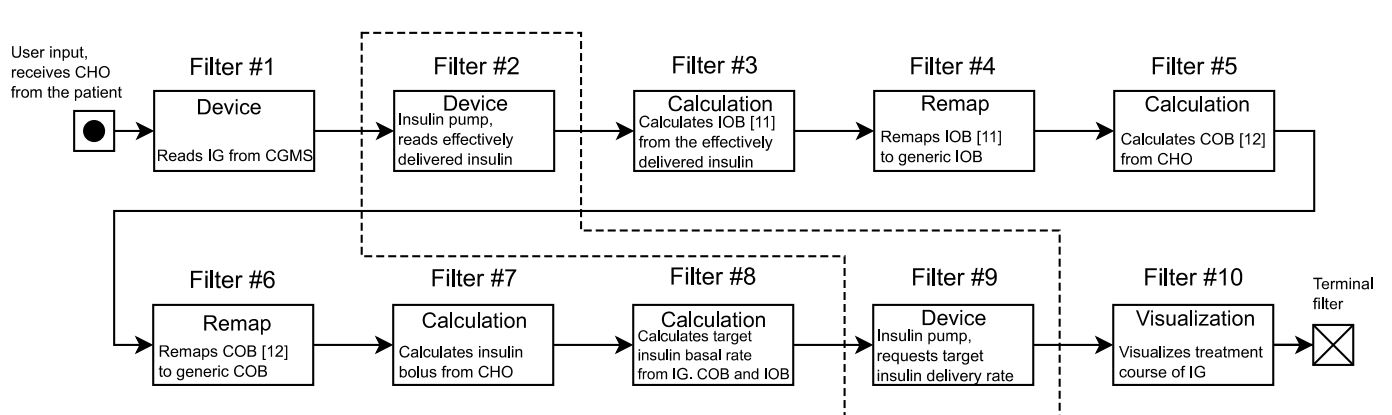
\includegraphics[width=1\textwidth]{img/scgms/filters.jpg}
\textit{Zdroj: SmartCGMS as an Environment for an Insulin-Pump  Development with FDA-Accepted In-Silico Pre-Clinical Trials \citep{cgms.ubl}}
\end{figure}

\textbf{Model} umožňuje načtení více hodnot voláním metody \textit{Get\_Continuous\_Levels} a jejich následné zpracování dle nastavených parametrů. Na rozdíl od filtru model zpracovává události dávkově. Je tak vhodný pokud potřebujeme pracovat s více signály najednou nebo predikovat hodnotu do budoucna. SmartCGMS obsahuje modely dynamiky glukózy Bergmanův model vylepšený Hovorkovo modelem a Koutného difúzním modelem, SimGlucose, s vynulovaným parametrem xi u UVA/Padova S2013, T1DMS a DMMS.R \citep{cgms.web}. Výpočet modelu je spušten filtrem \textit{Signal Generator} nebo filtrem \textit{Calculated Signal} pokud chceme  parametry modelu dynamicky spočítat pomocí solveru.

\textbf{Metrika} je druh filtru, který umožňuje spočítat metriky jako je například střední chyba, směrodatná odchylka nebo plocha pod křivkou \citep{cgms.koutny}.

Pro určení parametrů modelu lze využít \textbf{solver}. Ten na základě metrik signálů modelu spočítá jeho optimální parametry. Příkladem solveru je Meta-differential evolution, Pathfinder, Sequential brute force scan, Particle swarm optimization, Spiral optimization a další.

Vytvořené filtry, modely a solvery se zkompilují jako dynamické knihovna, která se načte při spuštění SmartCGMS. Aplikace také umožňuje integraci skriptů v jazyce Matlab. Skripty je nutné definovat v souboru \textit{matlab\_manifest.xml}.

SmartCGMS lze spustit v příkazové řádce (\textit{console3.exe}) nebo v grafickém uživatelském rozhraní (\textit{gpredict3.exe}). V záložce \textit{Filters} si uživatel nastaví jednotlivé filtry a jejich parametry. V záložce \textit{Simulation} pak spustí běh programu a může prohlížet grafy a logy s výstupy (příklad grafického výstupu je na obrázku \ref{fig:scgms_graf}). Konfiguraci lze uložit a poté opětovně načíst.

\begin{figure}[H]
\caption{Příklad výstupu SmartCGMS}
\label{fig:scgms_graf}
\centering
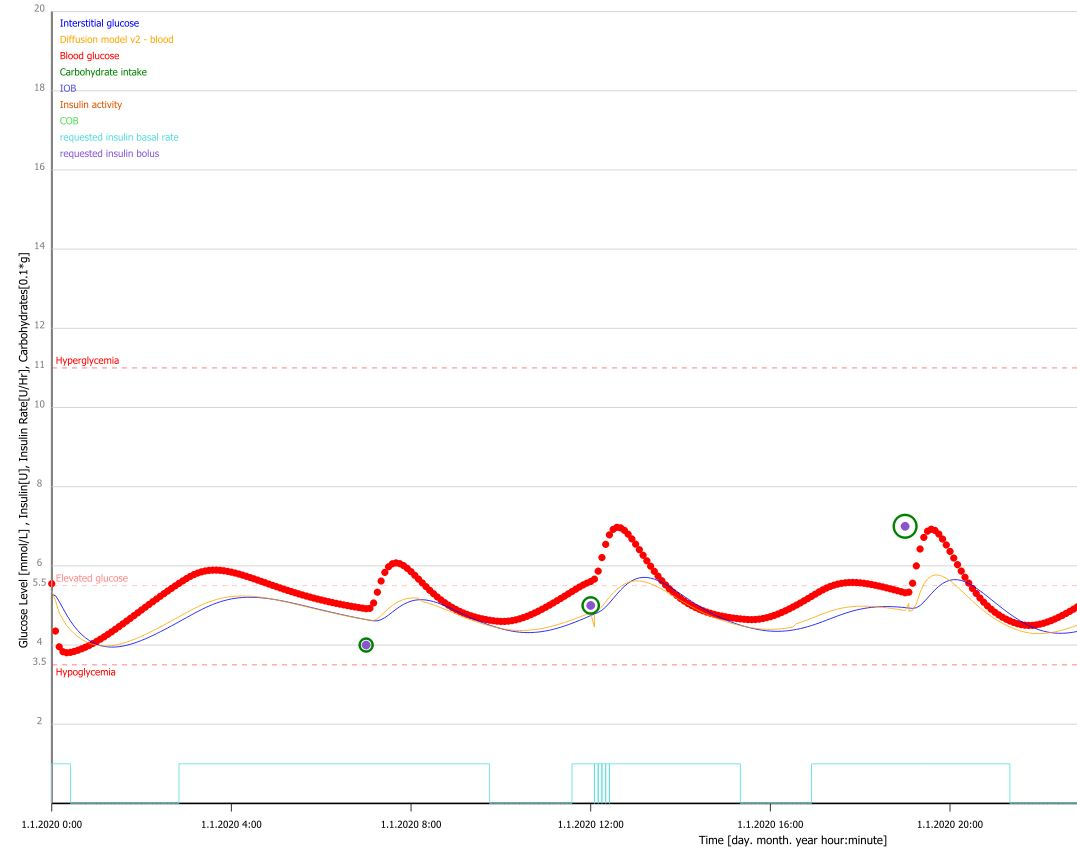
\includegraphics[width=1\textwidth]{img/scgms/graf1.jpg}
\textit{Zdroj: SmartCGMS}
\end{figure}

SmartCGMS je dostupný na \url{https://diabetes.zcu.cz/smartcgms}.
\chapter{Návrh metody detekce karbohydrátů}

Příjem karbohydrátů způsobuje zvýšení hladiny koncentrace glukózy v krvi, které je nutné kompenzovat podáním inzulinu. Včasnou detekcí může systém upravit množství podávaného inzulinu tak, aby nedošlo k hyperglykémii.

Detekce karbohydrátů je na základě dat intersticiální glukózy měřené senzorem CGMS a její derivace. Pro detekci jsem zvolil tyto 3 metody:
\begin{itemize}
\setlength\itemsep{0em}
\item Long short-term memory neuronová síť (kapitola \ref{ch:lstm})
\item Lineární a kvadratická diskriminační analýza (kapitola \ref{ch:lda_qda})
\item Detekce hran pomocí thresholdů 1. diference hodnot intersticiální glukózy \\(kapitola \ref{ch:threshold})
\end{itemize}

\section{Rekurentní neuronové sítě}
\label{ch:lstm}

Rekurentní neuronové sítě jsou vhodné pro predikci sekvenčních dat (například časové řady). Vyznačují se tím, že si předávají informaci o předchozím stavu (aktivaci skryté vrstvy):

$H_{t}=\sigma (W_{h}H_{t-1}+W_{x}X_{t}+b)$

\noindent kde $W$ jsou váhy a $b$ je bias. Neurony, které takto uchovávají svůj stav, se nazývají buňky. 

\begin{figure}[H]
\caption{Rekurentní neuronová síť}
\label{fig:rnn}
\centering
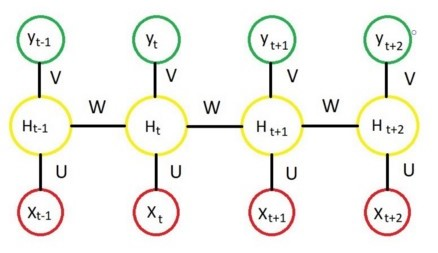
\includegraphics[width=0.65\textwidth]{img/cho/rnn.jpeg}\\
\textit{Zdroj: https://medium.com/}
\end{figure}

Riziko RNN spočívá v náchylnosti vzniku jevu označovaného jako mizející nebo explodující gradient vznikajícího při zpětné propagaci, kdy hodnoty exponenciálně klesají nebo rostou. To je z důvodu, že se chyba propaguje přes všechny iterace. Tento problém eliminuje long short-term memory nebo gated recurrent unit neuronová síť.

\subsection{Long short-term memory}

Long short-term memory neuronová síť (LSTM) je speciální případ rekurentní neuronové sítě. V každé iteraci si buňka uchovává dodatečnou informaci nazvanou \textit{memory}. 

Nejprve se ze vstupního vektoru $X_{t}$ a stavu předchozí buňky $H_{t-1}$ spočte Forget gate $f_{t}$, Candidate layer $\bar{C}_{t}$ Input gate $I_{t}$ a Output gate $O_{t}$ \citep{cho.lstm}:

$f_{t}=\sigma(X_{t} \otimes U_{f}+H_{t-1} \otimes W_{f})$\\\indent
$\bar{C}_{t}=tanh(X_{t} \otimes U_{c}+H_{t-1} \otimes W_{c})$\\\indent
$I_{t}=\sigma(X_{t} \otimes U_{i}+H_{t-1} \otimes W_{i})$\\\indent
$O_{t}=\sigma(X_{t} \otimes U_{u}+H_{t-1} \otimes W_{u})$

\noindent kde $W$ a $U$ jsou váhové vektory. Následně se spočte \textit{memory} prvek $C_{t}$:

$C_{t}=f_{t} \otimes C_{t-1} \oplus I_{t} \otimes \bar{C}_{t}$

\noindent a výstupní stav $H_{t}$:

$H_{t}=O_{t} \otimes tanh(C_{t})$

Diagram LSTM buňky je na obrázku \ref{fig:lstm_cell}.

\begin{figure}[H]
\caption{LSTM buňka}
\label{fig:lstm_cell}
\centering
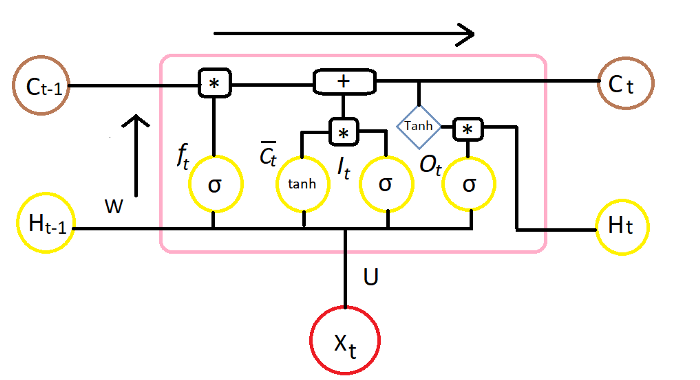
\includegraphics[width=0.9\textwidth]{img/cho/lstm_cell.png}
\textit{Zdroj: https://medium.com/}
\end{figure}

\subsection{Gated recurrent unit}

Gated recurrent unit neuronová síť (GRU) využívá Update gate $z_{t}$ a Reset gate $r_{t}$. Ty určují která informace bude propagována na výstup. Mohou tak vytěžit relevantní informace. Update a reset gate se spočte \citep{cho.gru}:

$z_{t}=\sigma(W_{z}x_{t} + U_{z}h_{t-1})$\\\indent
$r_{t}=\sigma(W_{r}x_{t} + U_{r}h_{t-1})$

\noindent kde $W$ a $U$ jsou váhové vektory. Následně se spočte relevantí informace z předchozího stavu $\bar{h}_{t}$:

$\bar{h}_{t}=tanh(W_{h}x_{t} + U_{h}(r_{t} \otimes h_{t-1}))$

\noindent a výstupní stav $h_{t}$:

$h_{t}=z_{t} \otimes h_{t-1} + (1-z_{t}) \otimes \bar{h}_{t}$

Diagram GRU buňky je na obrázku \ref{fig:gru_cell}.

\begin{figure}[H]
\caption{GRU buňka}
\label{fig:gru_cell}
\centering
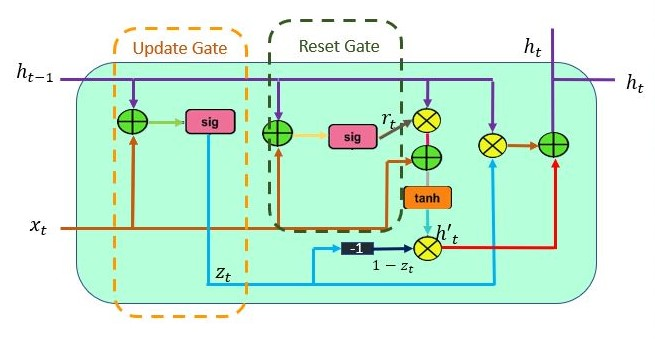
\includegraphics[width=1\textwidth]{img/cho/gru_cell.jpg}
\textit{Zdroj: https://www.pluralsight.com/}
\end{figure}

\subsection{Model}

Pro detekci karbohydrátů jsem sestavil sekvenční keras model\footnote{Keras je nadstavba nad knihovnou TensorFlow pro neuronové sítě} se čtyřmi vrstvami:
\begin{itemize}
\setlength\itemsep{0em}
\item Obousměrná LSTM nebo GRU
\item Dropout(0,5)
\item Dense(128)
\item Dense(1)
\end{itemize}

První vrstvou je rekurentní neuronová síť. Ta může být buď LSTM nebo GRU. Tato vrstva má 128 neuronů, dropout 0,2 a aktivační funkcí je hyperbolický tangens. Vstupem vrstvy je časové okno N vstupních prvků velikosti W. Tvar vstupních dat je WxN:

$\begin{bmatrix}
X^{1}_{1} & X^{2}_{1} & ... & X^{N}_{1}\\
X^{1}_{2} & X^{2}_{2} & ... & X^{N}_{2}\\
... & ... & ... & ...\\
X^{1}_{W} & X^{2}_{W} & ... & X^{N}_{W}
\end{bmatrix}$

Dropout vrstva s \textit{rate=0,2} náhodně nastaví některé vstupy na nulu v poměru 0,2. Nevynulované vstupy jsou škálovány 1/(1-rate), takže součet všech vstupů je nezměněn. To zabrání přetrénování neuronové sítě. Droupout vrstva je aplikována pouze při trénování sítě. První Dense vrstva (propojení neuronů formou každý s každým) má 128 neuronů, aktivační funkce je \textit{relu}. Druhá Dense vrstva s jedním neuronem je výstupní.


\section{Lineární a kvadratická diskriminační analýza}
\label{ch:lda_qda}

Pro diskriminační analýzu jsem se rozhodl vzhledem k vysoké úspěšnosti a malému zpoždění, které dosáhli \citet{analyzaCHO.LDA} v článku \textbf{Pattern Recognition Reveals Characteristic Postprandial Glucose Changes: Non-Individualized Meal Detection in Diabetes Mellitus Type 1} (kapitola \ref{ch:analyzaCHO:lda}).

Diskriminační analýza slouží k rozdělení prvků do konečného počtu tříd na základě lineární kombinace charakteristických prvků. Pro klasifikaci potřebujeme znát posteriory tříd \textbf{P(Y|X)}. Pravděpodobnostní model \textbf{P(X|y=k)} pro každou třídu \textbf{k} lineární a kvadratické diskriminační analýzy je dán vícerozměrnou Gaussovo distribucí \citep{cho.book.lda}:

\scalebox{1.2}{$P(X|y=k)=\frac{1}{(2\pi)^{p/2}|\sum_{k}|^{\frac{1}{2}}}e^{-\frac{1}{2}(x-\mu_{k})^{T}\sum^{-1}_{k}(x-\mu _{k})}$}\\\\
kde \textbf{p} je počet prvků. Pro predikci je pak použito Bayesovo rozhodovací pravidlo \citep{cho.book.lda}:

\scalebox{1.2}{$P(y=k|x)=\frac{P(x|y=k)P(y=k)}{P(x)}=\frac{P(x|y=k)P(y=k)}{\sum_{l}{P(x|y=l)P(y=l)}}$}\\\\
kdy hledáme třídu s maximálním posteriorem.

Logaritmus posterioru pro kvadratickou diskriminační analýzu (QDA) je \citep{cho.book.lda}:

$P(y=k|x)=-\frac{1}{2}log|\sum_{k}|-\frac{1}{2}(x-\mu_{k})^{T}\sum^{-1}_{k}(x-\mu_{k})+logP(y=k)$\\\\
Predikovaná třída je ta, která má maximální logaritmický posterior.

Lineární diskriminační analýza (LDA) je speciální případ QDA, kdy předpokládáme, že třídy mají stejnou kovarianční matici. Logaritmus posterioru je pak vyjádřen \citep{cho.scikit.lda}:

$P(y=k|x)=-\frac{1}{2}(x-\mu_{k})^{T}\sum^{-1}(x-\mu_{k})+logP(y=k)$\\

Vstupem diskriminační analýzy může být buď množina prvků pro daný časový okamžik nebo časové okno jednoho prvku. Predikované třídy jsou příjem/nepříjem karbohydrátů. Ty dostaneme převedením sloupce karbohydrátů na booleanovskou proměnnou (0 je false, cokoli větší než 0 je true).

\subsection{Množina prvků}

Nejčastějším vstupem diskriminační analýzy je množina charakteristických prvků $X_{i}$. V tomto případě se diskriminační analýza snaží rozdělit prostor tak, aby odlišila jednotlivé třídy (viz obrázek \ref{fig:lda}).

\begin{figure}[H]
\caption{Rozdělení prostoru lineární diskriminační analýzou dvou prvků}
\label{fig:lda}
\centering
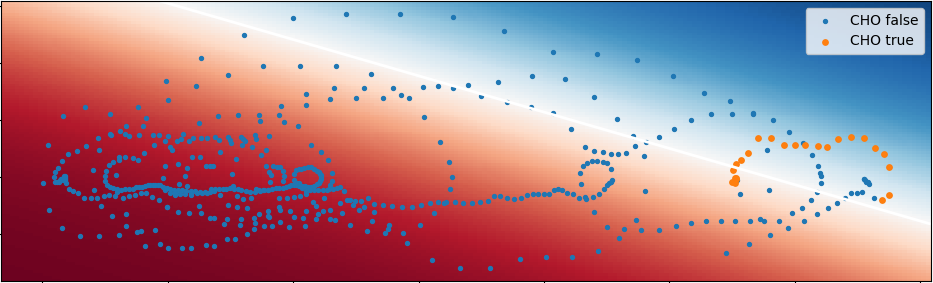
\includegraphics[width=1\textwidth]{img/cho/lda2.png}
\end{figure}

\subsection{Časové okno}

V případě časového okna muže být na vstupu pouze jediný prvek. To je dáno tím, že vstupem diskriminační analýzy je jedno-dimenzionální pole dat. Vstupní data mají tvar:

$\begin{bmatrix}
X_{i-W} & X_{i-W-1} & ... & X_{i-1} & X_{i}
\end{bmatrix}$

\noindent kde W je velikost časového okna. Časové okno jako vstupní data použili i \citet{analyzaCHO.LDA}.

Při experimentální implementaci diskriminační analýzy se mi nepodařilo dosáhnout stejných výsledků, jako autoři původního článku. Nejlepších výsledků dosahoval kvadratická diskriminační anaýza jejímž vstupem bylo dvou hodinové časové okno. Z testovacích 150 zadaných jídel jich detekovala 54 \% a falešně pozitivních detekcí bylo 155. Rozdílné výsledky mohou být dány tím, že původní metoda byla otestována pouze s daty predikovanými na základě Bergmanova modelu, ale ne s reálnými daty pacientů.

\section{Detekce hran průběhu intersticiální glukózy}
\label{ch:threshold}

Tato metoda detekuje vzestupné a klesající hrany průběhu intersticiální glukózy pomocí thresholdů první diference měřených hodnot intersticiální glukózy.

Derivace funkce $f'(x)$ v bodě $x$ je směrnicí tečny funkce $f(x)$ v daném bodě. Její hodnota je rovna tangens úhlu $\alpha$, který tečná svírá s osou x. Pakliže je funkce $f(x)$ v bodě $x$ rostoucí, $tg(\alpha)$ je kladný. Pokud je $f(x)$ klesající, $tg(\alpha)$ je záporný. Velikost derivace v bodě $x$ pak udává velikost změny $f(x)$, neboli říká, jak strmě funkce stoupá či klesá. Derivace funkce $f(x)$ v bodě $x_{1}$ můžeme vyjádřit jako:

\scalebox{1.2}{$f'(x) = \frac{d}{dx}f(x) = \lim_{x \to x_{0}} \frac{f(x)-f(x_{0})}{x-x_{0}}$}

Jelikož data ze senzoru CGMS jsou diskrétní, můžeme derivaci nahradit rovnicí první diference. Pro data intersticiální glukózy tak dostáváme vztah:

\scalebox{1.2}{$\Delta IST = \frac{IST_{t} - IST_{t-1}}{\Delta t}$}

Naměřená data intersticiální glukózy mohou být zatížena šumem a případně i dočasnými výchylkami hodnot glukózy. Každá taková výchylka pak má značný vliv na hodnotu derivace. Z toho důvodu je potřeba data před výpočtem vyhladit. Pro vyhlazení dat byl zvolen digitální Savitzky-Golay filtr. Každá podmnožina $2m+1$ prvků je vzorkována na polynom stupně $p (p\leq 2m)$ ve smyslu nejmenších čtverců \citep{cho.savgol}. Pro vyhlazení dat intersticiální glukózy jsem zvolil polynom stupně 3 a velikost podmnožiny 21. Vyhlazená data vidíme v grafu na obrázku \ref{fig:savgol}.

\begin{figure}[H]
\caption{Vyhlazená data intersticiální glukózy}
\label{fig:savgol}
\centering
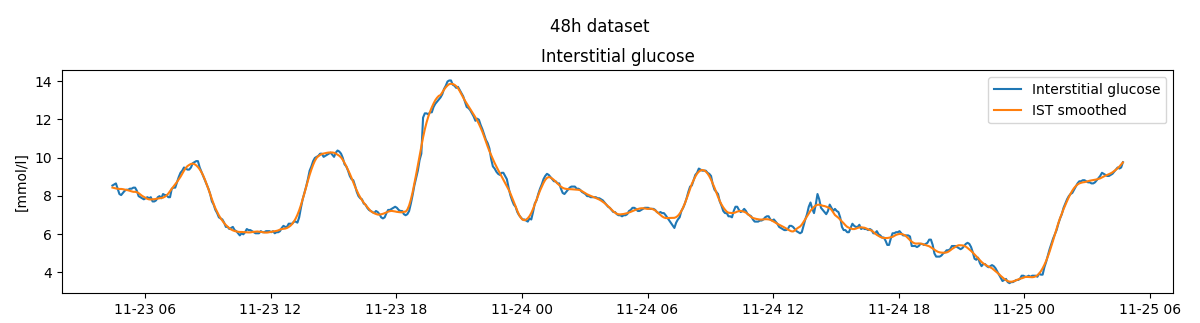
\includegraphics[width=1\textwidth]{img/cho/savgol.png}
\end{figure}

Následně se data ohodnotí. Pokud $\Delta IST$ překročí určitý threshold $th_{i}$, přiřadí se váha $w_{i}$. Takových dvojic thresholdů a vah může být libovolné množství. Experimentálně byla zjištěna kombinace thresholdů $th=[0.0125, 0.018]$ a vah $w=[2.25, 3]$.

Samotné ohodnocení podle thresholdů zachytí jakýkoli jednorázový větší výkyv v datech intersticiální glukózy. Jelikož příjem karbohydrátů se projevuje zvýšením glykémie v řádu desítek minut až hodin, chceme znát vývoj křivky intersticiální glukózy v čase. Z toho důvodu pro kladně ohodnocená data zvýšíme ohodnocení v případě, že předchozí hodnoty vykazují vzrůstající trend po dobu dvou hodin nazpět (tj. 24 hodnot, data jsou vzorkována po pěti minutách). Získáme tak aktivační funkci pro rostoucí hrany.
\begin{verbatim}
if activation[i] > 2:
  for j in range(24):
    if activation[i-j] >= 2+0.2*j:
      activation[i] += 0.1*j
\end{verbatim}
Pro klesající hrany použijeme stejný postup, ale se záporným ohodnocením.

V grafu na obrázku \ref{fig:hrany} je ukázka detekce hran. Červeně je aktivace vzestupné hrany, modře aktivace sestupné hrany posunuté. Počátek sestupné hrany je posunut na úrověň poslední hodnoty aktivace vzestupné hrany. Mezi vzestupnou a sestupnou hranou je vždy několik hodnot, kdy byla hladina intersticiální glukózy vyrovnaná.

\begin{figure}[H]
\caption{Detekované hrany průběhu intersticiální glukózy}
\label{fig:hrany}
\centering
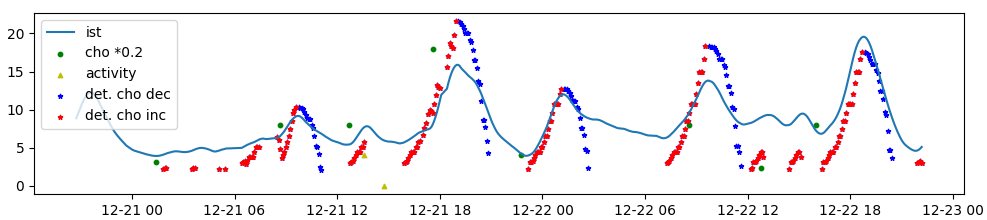
\includegraphics[width=1\textwidth]{img/cho/hrany.png}
\end{figure}

Jídlo je detekováno, pakliže aktivační funkce vzestupné hrany je větší než zvolený threshold. Nízký threshold detekuje většinu jídel, ale také může detekovat výkyvy nesouvisející s příjmem karbohydrátů. Naopak vysoce zvolený threshold nebude detekovat menší jídla. Řešením je použití více thresholdů pro stanovení pravděpodobnosti jídla.
\chapter{Návrh metody detekce fyzické aktivity}
\chapter{Implementace}

\section{Použité nástroje}

Při návrhu metod jsem používal jazyk Python, který je vhodný pro analýzu dat, zvláště pak jeho knihovny NumPy, Pandas a SciPy pro zpracování a analýzu dat a matplotlib pro vykreslení dat. Dále jsem použil knihovny TensorFlow a Keras pro práci s neuronovými sítěmi a knihovnu Scikit-learn pro strojové učení.

Implementace modulů do SmartCGMS je v jazyce C++. Použití Keras modelu neuronové sítě je za pomoci knihovny frugally-deep\citep{cho.frugally}.

\section{Dataset BGLP}
\label{ch:bglp}

\begin{setlength}{\parskip}{0pt}
Anonymizovaná data ze senzoru CGMS obsahují naměřené a zadané hodnoty:
\begin{itemize}
\setlength\itemsep{0em}
\item Glukóza v krvi (BG)
\item Intersticiální glukóza (IST)
\item Bazální množství inzulinu
\item Bolus inzulinu
\item Příjem karbohydrátů (CHO)
\item Fyzická aktivita
\item Kvalita spánku
\item Elektrodermální aktivita
\item Teplota kůže
\item Teplota okolí
\item Srdeční tep
\item Počet kroků
\item Akcelerace
\end{itemize}
\end{setlength}

Intersticiální glukóza je měřena v pětiminutových intervalech. Glukóza v krvi, podávaný inzulin (bolus i bazál), karbohydráty, fyzická aktivita a kvalita spánku jsou zadávány pacientem. Senzor měří buď srdeční tep a počet kroků, nebo akceleraci. Srdeční tep a počet kroků se měří v pětiminutových intervalech, akcelerace v minutových intervalech. Elektrodermální aktivita a teplota kůže a okolí se měří ve stejném intervalu podle toho, zda se měří tep nebo akcelerace.

\begin{setlength}{\parskip}{0pt}
CGMS senzor posílá data ve formě signálů, které mají strukturu:
\begin{itemize}
\setlength\itemsep{0em}
\item Logical Clock
\item Device Time
\item Event Code
\item Signal
\item Info
\item Segment Id
\item Event Code Id
\item Device Id
\item Signal Id
\end{itemize}
\end{setlength}

Příklad signálů ze senzoru CGMS je v tabulce \ref{tab:cgms_data}. Informaci pro následnou detekci v sobě nesou sloupce Device Time (čas měření), Signal (typ signálu) a Info (hodnota).

\begin{table}[H]
\caption{Signály ze CGMS}
\label{tab:cgms_data}
\centering
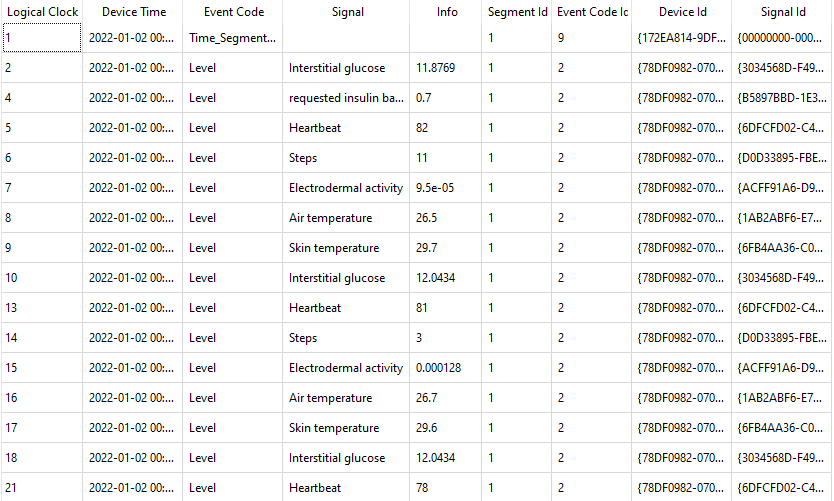
\includegraphics[width=1\textwidth]{img/cho/cgms_data.png}
\end{table}

V grafech na obrázku \ref{fig:48h_dataset} jsou transformovaná data naměřená senzorem CGMS za 48 hodin. Na prvním grafu jsou hodnoty Intersticiální glukózy a její vyhlazení Savitzky-Golay filtrem. Druhý graf znázorňuje zadanou bazální dávku inzulinu, bolusy, příjem karbohydrátů a fyzickou aktivitu. Na posledním grafu jsou hodnoty srdečního tepu, počtu kroků, elektrodermální aktivity, teploty kůže a teploty okolí.

\begin{figure}[H]
\caption{Data ze CGMS}
\label{fig:48h_dataset}
\centering
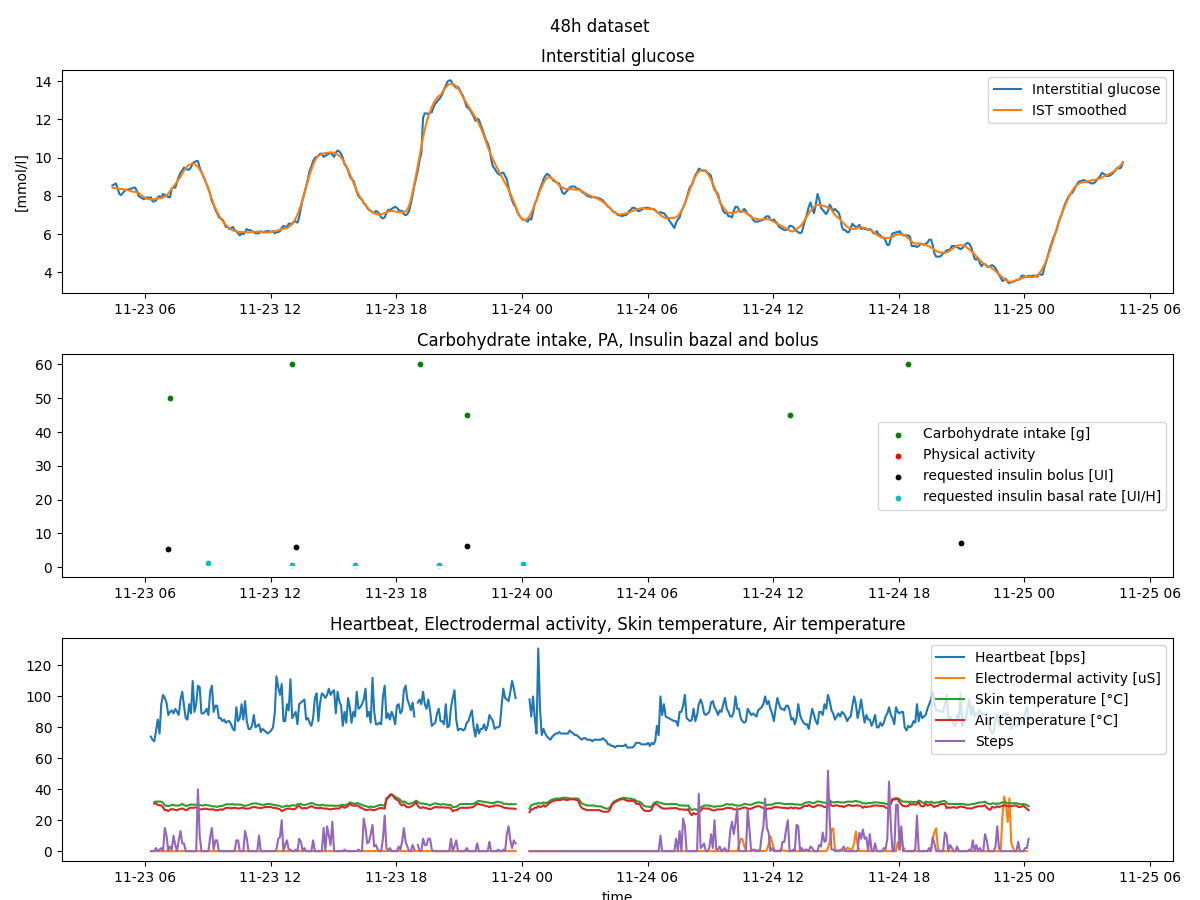
\includegraphics[width=1\textwidth]{img/cho/48h_dataset.png}
\end{figure}


\section{Filtr pro SmartCGMS}

Algoritmy jsou do SmartCGMS implementovány v podobě filtrů. Ty implementují rozhraní \textit{scgms::IFilter} a \textit{refcnt::IReferenced}. Při vytvoření instance filtru se volá metoda \textit{Configure}, která slouží pro nastavení filtru (typicky přečtení a nastavení konfiguračních parametrů). Metoda \textit{Execute} je volána pokaždé, když přijde signál od předchozího filtru. Tato metoda vykonává požadovanou funkcionalitu. Původní událost se na závěr zpravidla posílá dalšímu filtru. Současně se musí zaregistrovat descriptor nového filtru, který definuje ID filtru, název a konfigurační parametry, a případně i descriptor nového signálu. Vytvořená dynamická knihovna musí exportovat funkce \textit{do\_create\_filter}, \textit{do\_get\_filter\_descriptors} a \textit{do\_get\_signal\_descriptors}.

Data mohou být rozdělena do časových segmentů dle měření. V takovém případě filtry pracují s každým segmentem zvlášť. Rozdělení do segmentů je realizováno pomocí mapy, kdy klíčem je ID segmentu a hodnotou datová struktura pro daný filtr. Na konci segmentu se údaj z mapy vymaže.

Implementované algoritmy pracují s daty v určitém časovém okně. Pro tyto účely jsem vytvořil vlastní spojový seznam na principu klouzavého okénka \textbf{swl}. Ten dědí od \textit{std::deque}, které umožňuje vkládání prvků z obou stran i indexaci. Konstruktor má jeden parametr určující velikost okna. Při vložení nadlimitního prvků se odebere prvek z druhého konce seznamu.

Pro vyhlazení dat jsem implementoval \textbf{Savitzky-Golay} filtr. Tomuto filtru se nastavuje typ signálu, který má vyhladit, velikost okna a stupeň polynomu. Výstupem je \textbf{IST smoothed} signál.

Pro vyhodnocení úspěšnosti detekce je implementován \textbf{Evaluate} filtr. Tento filtr neřeší časové segmenty. Nastavit lze zkoumaný a referenční signál, časové okno pro detekci, cooldown pro započtení falešně pozitivního výsledku a minimální počet referenčních aktivit za den. Filtr započítává dvě úrovně detekovaného signálu. Nižší (1) pro detekované aktivity a vyšší (2) pro potvrzení. Filtr zaznamenává výsledky pro každý den. Pokud počet referenčního signálu je menší, než minimální počet, den se nezapočte do celkového součtu.

Možnosti nastavení všech filtrů a spuštění detekce je popsáno v příloze B.


\subsection{Detekce příjmu karbohydrátů}

\textbf{CHO detection} filtr počítá aktivační funkci a detekci karbohydrátů. To je implementováno rekurentní neuronovou sítí nebo detekcí hran průběhu intersticiální glukózy tak jak je popsáno v kapitole \ref{ch:threshold}. Filtr posílá dva signály. \textbf{Activation} signál je výstup použitého algoritmu a \textbf{CHO probability} udávající detekovaný příjem (1 - nižší pravděpodobnost, 2 - vyšší pravděpodobnost).

V případě detekce hran jsou nastaveny 2 thresholdy. Nižší pro brzkou detekci, která ale může detekovat výkyvy nesouvisející s příjmem jídla. Vyšší threshold je potvrzovací, kdy existuje vysoká pravděpodobnost příjmu karbohydrátů. Detekce je pouze pro vzestupnou hranu. Potvrzení může být i pomocí rekurentní neuronové sítě. Příklad konfigurace thresholdů je v konfiguračním souboru \texttt{setup\_th.ini} (viz příloha B). V případě detekce hran musí tomuto filtru předcházet Savitzky-Golay filtr pro vyhlazení dat intersticiální glukózy.

\subsubsection{Rekurentní neuronová síť}

Rekurentní neuronová síť využívá natrénovaného keras modelu.Ten je možné použít v C++ pomocí knihovny frugally-deep \citep{cho.frugally}.

Před trénováním modelu je třeba data ve formě signálů transformovat. Sloupce Device Time, Signal a Info jsem extrahoval do dvourozměrné tabulky, kde řádky jsou čas měření a sloupce jednotlivé typy signálů. Jelikož různé typy signálu nejsou měřeny ve stejný okamžik, řádky jsem seskupil podle sloupce intersticiální glukózy, která je měřena v pětiminutových intervalech. Data intersticiální glukózy jsem interpoloval Akima spline \citep{cho.akima}, z níž jsem získal chybějící hodnoty a derivace 1. 2. a 3. řádu.

Model může být natrénován individuálně pro každého pacienta, nebo na celém souboru dat. Vstupní data modelu jsou hodnoty intersticiální glukózy, jejich první derivace a čas signálu v minutách. Díky časovému údaji neuronová síť zahrne do predikce určité denní návyky pacienta. Časové okno je velikosti 24 (tj. 2 hodiny). Z datasetu je 80 \% dat použito pro trénování a 20 \% pro validaci. Data jsou do neuronové sítě dávkována v dávkách o velikosti 64. Jelikož se jedná o časovou řadu, data se nepromíchávají. Jako ztrátová funkce je použita střední kvadratická chyba (MeanSquaredError), optimalizační algoritmus je Adam. Neuronová síť je trénovaná ve 100 epochách. 

Natrénovaný model je nutné konvertovat pomocí skriptu \texttt{keras\_export/ convert\_model.py}, který je součástí frugally-deep knihovny. Podporované sítě jsou LSTM i GRU. SmartCGMS filtr následně tento model načte při konfiguraci. Příklad konfigurace s GRU je v konfiguračním souboru \texttt{setup\_gru.ini} (viz příloha B).



\subsection{Detekce fyzické aktivity}

Filtr \textbf{PA detection} detekuje fyzickou aktivitu na základě vybraných ukazatelů nebo jejich kombinace. Detekce probíhá z poslední hodnoty naměřené senzorem, nebo průměru více hodnot dle zvoleného časového okna. Pro každý ukazatel lze zadat threshold.

Pro detekci sestupné hrany je nutné před tento filtr zařadit \textit{Savitzky-Golay} filtr pro vyhlazení dat. Nastavení thresholdů a vah je stejné jako u detekce karbohydrátů.


V případě, že se nepoužívá potvrzení detekcí sestupné hrany, posílá filtr signál \textbf{PA detected} o hodnotě 2. Při použití detekce sestupné hrany má tento signál hodnotu 1 pokud byla aktivita detekována pouze na základě ukazatelů a hodnotu 2 pokud byla detekce potvrzena sestupnou hranou.

Příklad konfigurace s měřeným srdečním tepem a počtem kroků je v konfiguračním souboru \texttt{setup\_bpm.ini}. Příklad konfigurace s akcelerací a potvrzováním pomocí detekce sestupné hrany je v konfiguračním souboru \texttt{setup\_acc.ini} (viz příloha B).
\chapter{Výsledky}

Algoritmy byly testovány na datech jedenácti pacientů. Měření testovacích dat u každého pacienta probíhalo po dobu 10 - 11 dnů. V součtu pacienti zaznamenali 340 jídel za 109 dnů. Výsledky pro jednotlivé pacienty jsou v souboru \textit{results.txt}. V tabulce \ref{tab:results} jsou souhrnné výsledky detekce karbohydrátů.

Pravdivě pozitivní (TP) jsou hodnoty, kdy je jídlo detekováno (hodnota detekce alespoň 1) do dvou hodin od jeho zadání pacientem. Pokud je hodnota detekce 2, je jídlo bráno jako potvrzeno. Pakliže jídlo není detekováno do dvou hodin od zadání, je výsledek falešně negativní (FN). V případě detekce hodnoty 2, kdy jídlo není zadané, výsledek je falešně pozitvní (FP). Zároveň je počítáno zpoždění detekce od zadání jídla pacientem. Jelikož v datech nemusí být některá jídla zadaná, statistika každého dne se započítá pouze tehdy, kdy byly zadány alespoň 3 jídla.

\begin{table}[H]
\caption{Výsledky}
\label{tab:results}
\begin{tabular}{|l|c|c|c|}
\hline 
& \textbf{Detekce hran} & \textbf{Detekce hran+GRU} & \textbf{ GRU }\\
\hline 
\hline 
Jídel & 340 &  &  \\\hline
Úspěšnost & 85 \% &  &  \\\hline
TP & 289 &  &  \\\hline
TP/pacient & 26,27 &  &  \\\hline
TP potvrzeno & 167 &  &  \\\hline
Potvrzeno & 57,8 \% &  &  \\\hline
FN & 45 &  &  \\\hline
FN/pacient & 4,09 &  &  \\\hline
FP & 112 &  &  \\\hline
FP/pacient & 10,18 &  &  \\\hline
Zpoždění* & 27,54 &  &  \\
\hline
\end{tabular}
\begin{flushleft}
* průměrná doba detekce karbohydrátů od příjetí jídla v minutách\\
TP - true positive\\
FN - false negative\\
FP - false positive\\
\end{flushleft}
\end{table}

Průměrná úspěšnost detekce jídla je 85 \% s průměrným zpožděním 27,54 minut. Všechny algoritmy vykazují vysoký počet falešně pozitivních výsledků. To může být dáno častými výkyvy glukózy u pacienta nebo tím, že pacienti jídlo nezadávali poctivě, nebo ho zadali se zpožděním. Také prudké výkyvy koncentrace cukru v krvi spojené s jinou činností mouhou způsobit falešnou detekci. Zpoždění 27,54 minut je srovnatelné, nebo i lepší, než výsledky zkoumaných algoritmů v kapitole \ref{ch:analyzaCHO}.
\chapter{Závěr}

V rámci práce byly navrženy a implementovány metody detekce příjmu karbohydrátů pomocí rekurentních neuronových sítí a detekce hran průběhu intersticiální glukózy. Nejlepších výsledků dosahovala kombinace detekce hran a rekurentní neuronové sítě, kdy citlivost detekce byla 89 \%. Zpoždění detekce 22,61 minut je srovnatelné, nebo i lepší, než výsledky zkoumaných algoritmů v kapitole \ref{ch:analyzaCHO}.

Metoda detekce průběhu intersticiální glukózy by se dala za použití detekce vzestupné i sestupné hrany rozšířit pro detekci glykemického indexu.

Detekce fyzické aktivity je realizována na základě pohybových dat, srdečního tepu, elektrodermální aktivity a jejich kombinací. Nejvyšší citlivosti detekce bylo dosáhnuto při použití pohybových dat. Detekce sestupné hrany průběhu intersticiální glukózy neměla na výsledky vliv. Přesnost detekce fyzické aktivity by se dala zvýšit použitím 3-osého akcelerometru.

Metody detekce příjmu karbohydrátů i fyzické aktivity mají vyšší počet falešně pozitivních výsledků. To je dáno tím, že zkoumané ukazatele jsou ovlivněny mnoha externími faktory. V datech se také vyskytují oblasti, kdy pacient nezadal do aplikace poctivě všechny aktivity. U detekce karbohydrátů se množství falešně pozitivních detekcí podařilo snížit metodou potvrzování detekce vyšším thresholdem nebo neuronovou sítí. U detekce fyzické aktivity se falešně pozitivní výsledky značně snížily při použití kombinace ukazatelů.

Do aplikace SmartCGMS byly implementovány celkem čtyři filtry. Savitzky-Golay filtr pro vyhlazení dat, filtr detekce karbohydrátů umožňující detekci pomocí hran průběhu intersticiální glukózy, pomocí rekurentních neuronových sítí, nebo jejich kombinace, filtr detekce fyzické aktivity a evaluační filtr pro vyhodnocení výsledků.

Parametry filtrů jsou nastavitelné, pro ukázku bylo vytvořeno několik konfigurací. U detekčních filtrů jsou thresholdy ve formě parametrů modelu a je možné aplikaci rozšířit o solver, který by našel nejoptimálnější thresholdy pro každého pacienta.



\chapter*{Přehled zkratek}
\addcontentsline{toc}{chapter}{Přehled zkratek}

\begin{tabular}{ll}
BG & glukóza v krvi\\
CGM & kontinuální monitorace glukózy\\
CGMS & systém kontinuální monitorace glukózy\\
CHO & karbohydráty\\
IST & intersticiální glukóza\\
\\
CMHE & Commited moving horizon estimation\\
GRU & Gated recurrent unit neuronová síť\\
HMM & Hidden Markov model (Skrytý Markovův model)\\
LDA & lineární diskriminační analýza\\
LSTM & Long short-term memory neuronová síť\\
NN & neuronová síť\\
OC-SVM & one-class support vectore machine klasifikátor\\
PCA & metoda hlavních komponent\\
QDA & kvadratická diskriminační analýza\\
RelU & Rectified linear units funkce\\
RNN & rekurentní neuronová síť\\
\\
TP & pravdivě pozitivní\\
TN & pravdivě negativní\\
FN & falešně negativní\\
FP & falešně pozitivní\\
MAE & střední absolutní chyba\\
RMSE & střední kvadratické chyba\\
COD & koeficient determinace
\end{tabular}

\bibliographystyle{csplainnatkiv}
{\raggedright\small
\bibliography{literatura}
}

\chapter*{Příloha A: Tabulky}
\addcontentsline{toc}{chapter}{Příloha A: Tabulky}

\section*{Detekce karbohydrátů}

\begin{table}[H]
\caption{\textbf{Threshold}}
\vspace*{1mm}
\label{tab:vys:th}
\centering
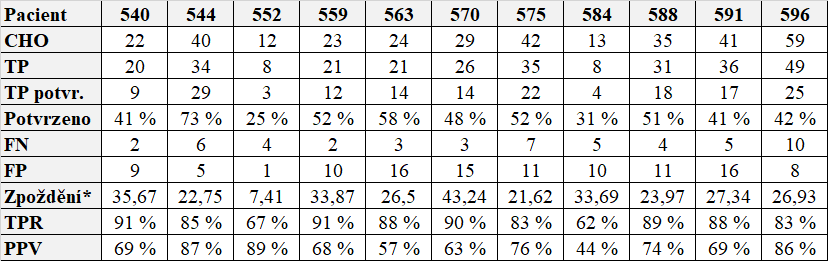
\includegraphics[width=1\textwidth]{img/vysledky/cho/1_th.png}
\end{table}

\begin{table}[H]
\caption{\textbf{GRU (individual)}}
\label{tab:vys:rnn_i}
\centering
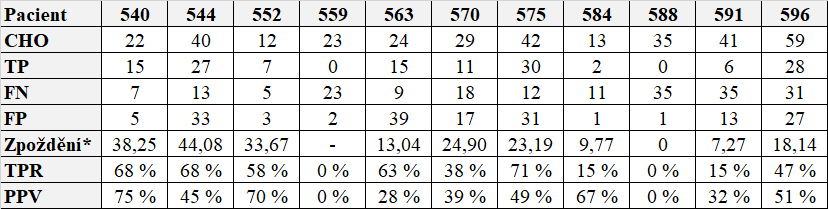
\includegraphics[width=1\textwidth]{img/vysledky/cho/2_rnn_i.png}
\end{table}

\begin{table}[H]
\caption{\textbf{Threshold + GRU (individual)}}
\label{tab:vys:thrnn_i}
\centering
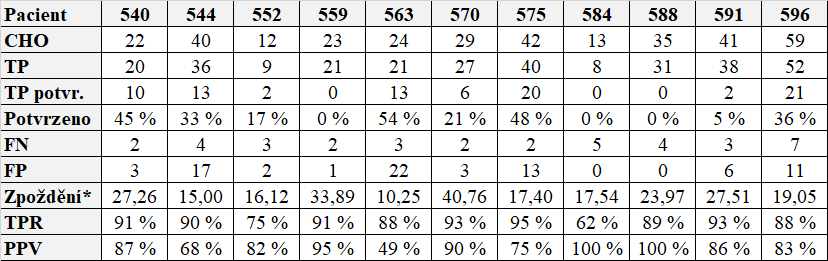
\includegraphics[width=1\textwidth]{img/vysledky/cho/3_thrnn_i.png}
\end{table}

\begin{table}[H]
\caption{\textbf{GRU}}
\vspace*{1mm}
\label{tab:vys:rnn}
\centering
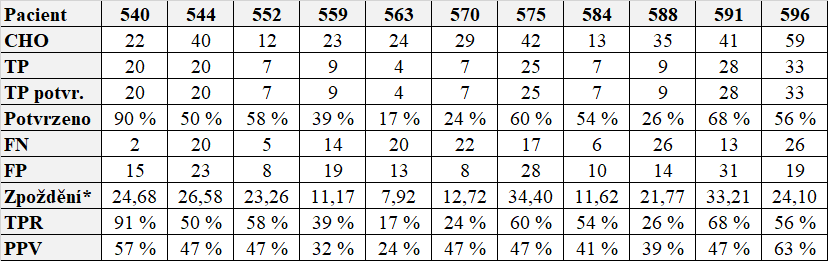
\includegraphics[width=1\textwidth]{img/vysledky/cho/4_rnn.png}
\end{table}

\begin{table}[H]
\caption{\textbf{Threshold + GRU}}
\label{tab:vys:thrnn}
\centering
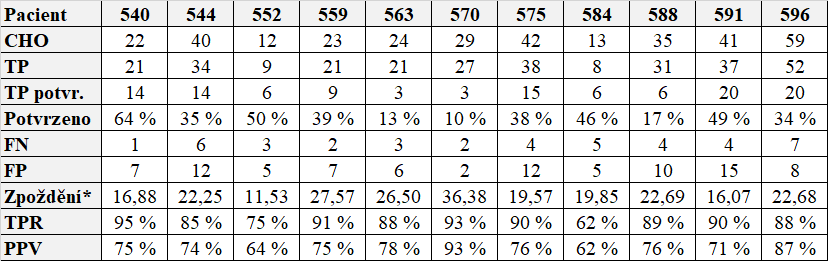
\includegraphics[width=1\textwidth]{img/vysledky/cho/5_thrnn.png}
\end{table}

\begin{table}[H]
\caption{\textbf{Souhrnné výsledky}}
\label{tab:vys:sum_cho}
\centering
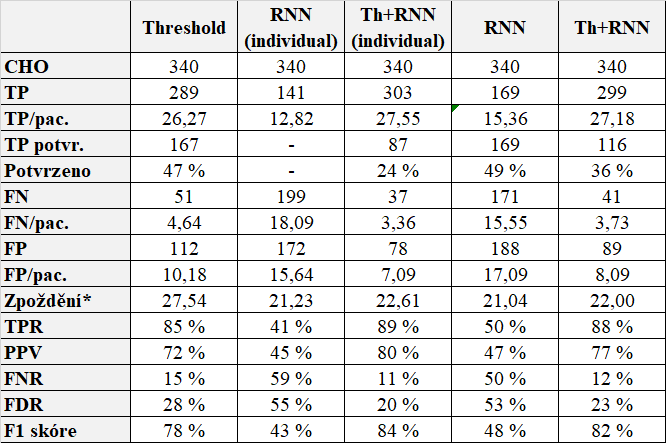
\includegraphics[width=0.9\textwidth]{img/vysledky/cho/cho.png}
\end{table}



\section*{Detekce fyzické aktivity}
\subsubsection*{Srdeční tep a počet kroků}

\begin{table}[H]
\caption{\textbf{Srdeční tep}}
\label{tab:vys:heart}
\centering
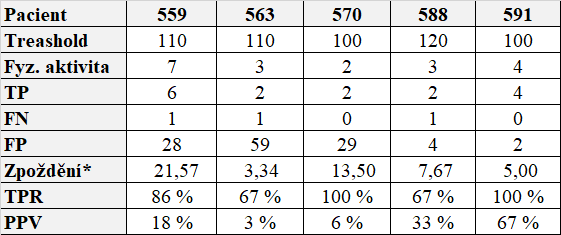
\includegraphics[width=0.8\textwidth]{img/vysledky/pa/1_heart.png}
\end{table}

\begin{table}[H]
\caption{\textbf{Počet kroků}}
\vspace*{1mm}
\centering
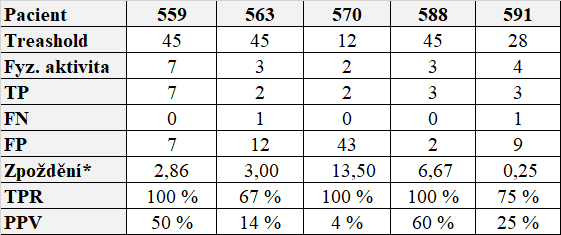
\includegraphics[width=0.8\textwidth]{img/vysledky/pa/2_steps.png}
\end{table}

\begin{table}[H]
\caption{\textbf{Elektrodermální aktivita}}
\vspace*{1mm}
\centering
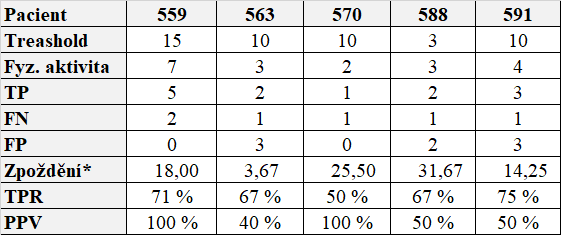
\includegraphics[width=0.8\textwidth]{img/vysledky/pa/3_elektro.png}
\end{table}

\begin{table}[H]
\caption{\textbf{Srdeční tep + počet kroků}}
\centering
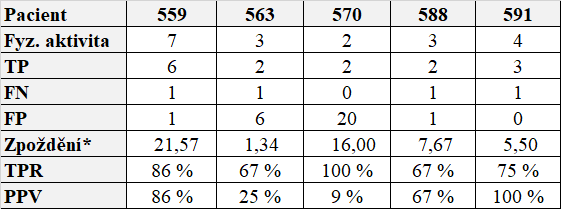
\includegraphics[width=0.8\textwidth]{img/vysledky/pa/4_heart_steps.png}
\end{table}

\begin{table}[H]
\caption{\textbf{Srdeční tep + elektrodermální aktivita}}
\centering
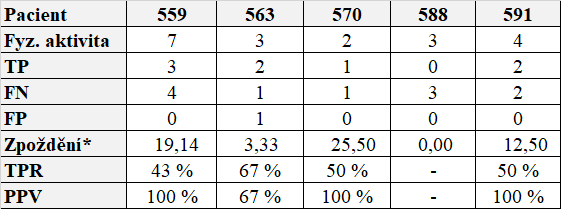
\includegraphics[width=0.8\textwidth]{img/vysledky/pa/5_heart_electro.png}
\end{table}

\begin{table}[H]
\caption{\textbf{Počet kroků + elektrodermální aktivita}}
\label{tab:vys:steps+}
\centering
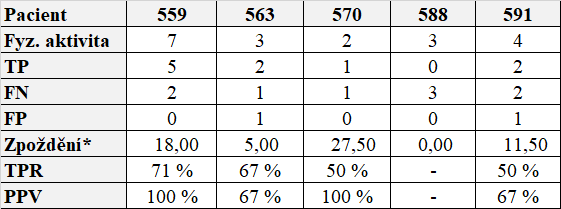
\includegraphics[width=0.8\textwidth]{img/vysledky/pa/6_steps_electro.png}
\end{table}

\begin{table}[H]
\caption{\textbf{Souhrnné výsledky}}
\label{tab:vys:sum_heart}
\centering
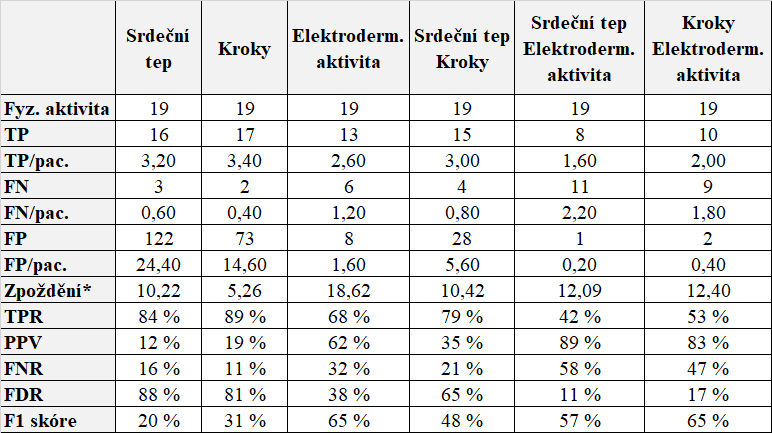
\includegraphics[width=1\textwidth]{img/vysledky/pa/vysledky 1.png}
\end{table}



\subsubsection*{Akcelerace}

\begin{table}[H]
\caption{\textbf{Akcelerace}}
\vspace*{1mm}
\label{tab:vys:acc}
\centering
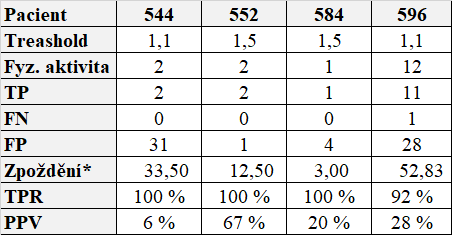
\includegraphics[width=0.7\textwidth]{img/vysledky/pa/7_acc.png}
\end{table}

\begin{table}[H]
\caption{\textbf{Elektrodermální aktivita}}
\vspace*{1mm}
\centering
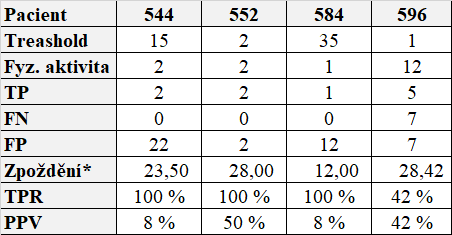
\includegraphics[width=0.7\textwidth]{img/vysledky/pa/8_electro2.png}
\end{table}

\begin{table}[H]
\caption{\textbf{Akcelerace + elektrodermální aktivita}}
\label{tab:vys:acc+}
\centering
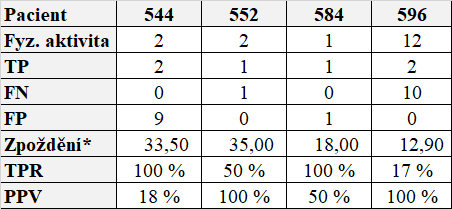
\includegraphics[width=0.7\textwidth]{img/vysledky/pa/9_acc_electro.png}
\end{table}

\begin{table}[H]
\caption{\textbf{Souhrnné výsledky}}
\label{tab:vys:sum_acc}
\centering
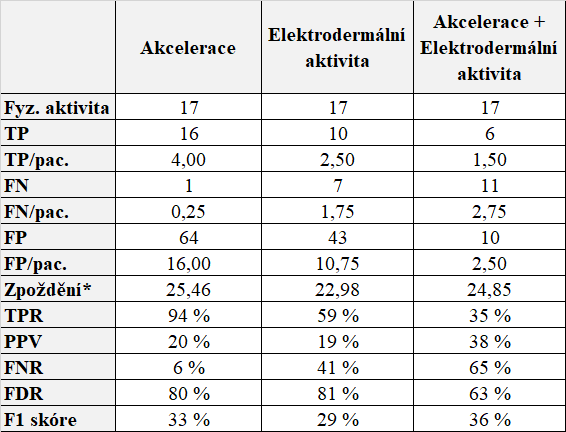
\includegraphics[width=0.8\textwidth]{img/vysledky/pa/vysledky 2.png}
\end{table}


\chapter*{Příloha B}
\addcontentsline{toc}{chapter}{Příloha B}

\section*{Adresářová struktura}
\addcontentsline{toc}{section}{Adresářová struktura}

\begin{itemize}
\item Aplikace\_a\_knihovny
 \begin{itemize}
  \item detection
  \begin{itemize}
  \item src - zdrojové soubory filtrů pro SmartCGMS
  \item CMakeLists.txt
  \end{itemize}
 \item lib - knihovny
 \item scripts - python skripty
 \item setup - konfigurační soubory
 \item detection.dll - knihovna filtrů pro SmartCGMS
 \end{itemize}
\item Poster
\item Text\_prace
 \begin{itemize}
  \item src - zdrojové tex soubory
  \item dp.pdf
  \end{itemize}
\item Vstupni\_data

 \begin{itemize}
  \item model - natrénované keras modely GRU sítě\\(vstupní data pacientů není možné přiložit z důvodu autorských práv)
  \end{itemize}
\item Vysledky - vysledky provedených experimentů
\end{itemize}

\section*{Knihovny, kompilace, spuštění}
\addcontentsline{toc}{section}{Knihovny, kompilace, spuštění}

SmartCGMS je dostupný na https://diabetes.zcu.cz/smartcgms. Knihovna je
kompilována v C++ 17. Pro kompilaci jsou nutné header soubory SmartCGMS
a knihovny \href{https://kinddragon.github.io/vld/}{VisualLeakDetector},
\href{https://github.com/Dobiasd/frugally-deep}{frugally-deep},
\href{https://gitlab.com/libeigen/eigen}{Eigen},
\href{https://github.com/Dobiasd/FunctionalPlus}{FunctionalPlus} a
\href{https://github.com/nlohmann/json}{json}. K dispozici je CMake
skript. Vytvořená dynamická knihovna \texttt{detection.dll} se umístí do
složky filters. Grafické rozhraní SmartCGMS se spustí programem
\texttt{gpredict3.exe}, konzolová verze programem \texttt{console3.exe}.

\section*{Nastavení filtrů}
\addcontentsline{toc}{section}{Nastavení filtrů}

\subsection*{Savitzky-Golay filtr}

Filtr pro vyhlazení dat.

\begin{itemize}
\setlength\itemsep{-1.5em}
\item Signal - zdrojový signál pro vyhlazení\\
\item Window size - velikost okna Savitzky-Golay filtru\\
\item Degre - stupeň polynomu
\end{itemize}

\noindent Filtr posílá vyhlazená data v signálu Savgol signal. V případě použití více filtrů je nutné výstupní signál přemapovat.

\subsection*{CHO detection}

Filtr detekce příjmu karbohydrátů.

\begin{itemize}
\setlength\itemsep{-1.5em}
\item Signal - detekovaný signál\\
\item Window size - velikost klouzavého okénka\\
\item Detect edges - detekce vzestupných hran\\
\item Detect descending edges - detekce sestupných hran\\
\item Rise threshold - threshold pro určení míry stoupání/klesání v čase\\
\item Use RNN - použití rekurentní neuronové sítě\\
\item RNN model file path - cesta k souboru s natrénovaným keras modelem převedeným do formátu pro frugally-deep\\
\item RNN threshold - threshold detekce neuronovou sítí\\
\item Thresholds\\
	\indent- Threshold Low - threshold malé změny IST\\
	\indent- Weight Low - váha malé změny IST\\
	\indent- Threshold High - threshold velké změny IST\\
	\indent- Weight High - váha velké změny IST
\end{itemize}

\noindent Filtr posílá aktivační funkce a detekované karohydráty.
Příklad konfigurace detekce hran průběhu intersticiální glukózy je v souboru \texttt{setup/setup\_th.ini}, příklad neuronové sítě v souboru \texttt{setup/setup\_gru.ini`}.

\subsection*{PA detection}

Filtr detekce fyzické aktivity.

\begin{itemize}
\setlength\itemsep{-1.5em}
\item Heartbeat - detekce podle srdečního tepu\\
\item Steps - detekce podle počtu kroků\\
\item Acceleration - detekce podle hodnoty akcelerace\\
\item Electrodermal activity - detekce podle elektrodermální aktivity\\
v Mean - použití průměru za časové okno\\
\item Window size - mean - velikost klouzavého okénka pro spočítání průměru (v případě velikosti okna 1 je průměr rovná aktuální hodnotě)\\
\item Detect IST edges - potvrzení detekce sestupnou hranou dat IST\\
\item Signal - detekovaný signal\\
\item Window size - edges - velikost klouzavého okénka pro detekci hran\\
\item Thresholds - threshold ukazatelů pro detekci a thresholdy a váhy pro detekci hran
\end{itemize}

\noindent Filtr posílá detekovanou fyzickou aktivitu.
Příklad konfigurace s měřeným srdečním tepem a počtem kroků je v konfiguračním souboru \texttt{setup/setup\_bpm.ini}. Příklad konfigurace s akcelerací a potvrzováním pomocí detekce sestupné hrany je v konfiguračním souboru \texttt{setup/setup\_acc.ini}.

\subsection*{Evaluation}

Filtr pro vyhodnocení výsledků.

\begin{itemize}
\setlength\itemsep{-1.5em}
\item Reference signal - referenční signál\\
\item Detected signál - detekovaný signál\\
\item Max detection delay - maximální zpoždění, které může mít detekovaný signál oproti referenčnímu\\
\item False positive cooldown - cooldown po detekci falešně pozitivního signálu, než je započítán další\\
\item Late detection delay - čas před referenčním signálem, kdy se bude detekce počítat jako pravdivě pozitivní\\
\item Min reference count - minimální počet referenčních signálů za den
\end{itemize}

\noindent Filtr na konci běhu simulace posílá info s naměřenými statistikami počtu referenčních signálů TP, potvrzené TP, FN, FP, zpoždění detekce a zpoždění potvrzení.

\section*{Python skripty}
\addcontentsline{toc}{section}{Python skripty}

Skripty umožňují transformaci a modifikaci dat BGLP, trénování
rekurentní neuronové sítě a analýzu metod detekce karbohydrátů a fyzické
aktivity. Pro spuštění skriptů je nutné mít nainstalovaný Python 3.7
nebo 3.8. Python 3.9 není podporovaný z důvodu nepodporované
kompatibilitě s knihovnou TensorFlow. Dále je nutné mít nainstalované
tyto balíčky: numpy, pandas, scipy, sklearn, tensorflow, tabulate, matplotlib, sweetviz.

V souboru \texttt{examples.py} jsou příklady práce se skripty:

\begin{itemize}
\itemsep1pt\parskip0pt\parsep0pt
\item lg.load\_log()- transformace dat z logu do csv
\item ld.load\_data() - modifikace dat pro detekci karbohydrátů nebo fyzické aktivity
\item cho.rnn() - trénování RNN
\item cho.lda() - LDA/GDA
\item cho.threshold() - detekce hran IST
\item pa.get\_feature() - spočtení vlastností (průměr, medián, směrodatná odchylka, rozdíl kvartilů)
\item pa.export\_features() - export vlastností do csv
\item pa.ML() - test metod strojového učení pro detekci fyzické aktivity
\end{itemize}

\subsection*{Trénování neuronové sítě}

Pro natrénování keras modelu rekurentní neuronové sítě je připraven skript \texttt{train\_rnn.py}. Ten se spouští příkazem \texttt{python train\_rnn.py\textless{}type\textgreater{} \textless{}options\textgreater{} {[}values{]}}, kdy \texttt{type} je typ neuronové \texttt{-gru} nebo \texttt{-lstm} (povinný parametr) a \texttt{options} jsou volitelné parametry: 

\noindent -f ~ název logu pacienta (* pro natrénování modelu na všech logách v adresáři)\\
 -i ~ adresář se vstupními logy (defaultně data/)\\
 -o ~ adresář pro uložení natrénovaného modelu (defaultně model/)\\
 -h ~ nápověda

\noindent Příklad natrénování GRU pro všechny pacienty: \texttt{python train\_rnn.py -gru -f * -i data/ -o model/} Příklad natrénování LSTM pro pacienta 575: \texttt{python train\_rnn.py -lstm -f 575-ws-training.log -i data/ -o model/}

\end{document}
